% Author - - Jon Arnt Kårstad, NTNU IMT
\documentclass{article}

% Importing document settings from our file "packages.sty"
\usepackage{packages}

% Beginning of document
\begin{document}

% Inserting title page
\import{./}{title}

% Defining front matter settings 
\frontmatter

% Inserting table of contents
\tableofcontents

% Inserting list of figures & list of tables
\listoffigures
\listoftables

% Defining main matter settings
\mainmatter

\section{Motivation}
    \import{./Sections/}{Motivation}

\section{Grundlagen}
    \import{./Sections/Introduction}{Introduction}

    \subsection{OOP Design Patterns}
        \import{./Sections/Introduction/OOPDesignPatterns}{OOPPatterns}

        \subsubsection{Observer}
            \import{./Sections/Introduction/OOPDesignPatterns/sub/}{Observer}

        \subsubsection{Proxy}
            \import{./Sections/Introduction/OOPDesignPatterns/sub/}{Proxy}

        \subsubsection{TemplateMethod}
            \import{./Sections/Introduction/OOPDesignPatterns/sub/}{TemplateMethod}

        \subsubsection{Builder}
            \import{./Sections/Introduction/OOPDesignPatterns/sub/}{Builder}

        \subsubsection{Facade}
            \import{./Sections/Introduction/OOPDesignPatterns/sub/}{Facade}
        \subsubsection{Singleton}
        \label{kap:gof:singleton}
            Mehr zu Singleton kann \textit{\textbf{Refactoring guru}} lesen.

            Singlteon garantiert, dass eine Klasse nur eine Instanz in der Anwendung hat.
            Dieser Pattern kann sehr hilfreich sein, wenn man weißt, man hat nur eine Instanz der Klasse im Programm 
            und auf sie möchte man aus allen Stellen der Anwendung zugreifen.
            Das Verhalten ähnelt sich mit dem Verhalten einer 
            globalen Variable deren Wert (die erstellte Instanz) nicht ersetzt werden kann.

            Ein großes Nachteil bei der Benutzung des Singletons ist, 
            dass die Teile des Programms, in denen Singleton aufgerufen wird, nicht unabhängig von ihm getestet werden können.
        \subsubsection{Abstract Factory}
            some info to abstract factory

    \subsection{Architecturen}
        \subsubsection{Clean Architectur}
            \import{./Sections/Introduction/CleanArchitecture}{CleanArchitecture}
        \newpage
        \subsubsection{Model-View-Presenter Architektur}
            Mehr zu MVP (Model-View-Presenter) kann man \textit{\textbf{in folgende Quelle}} lesen.

            Model-View-Presenter Architektur wird in den Anwendungen benutzt, die eine Oberfläche besitzen.
            Die Architektur teilt die Anwendung in 3 Teile:
            \begin{itemize}
                \item \textbf{Model} - enthält die komplete Logik des Programms.
                \item \textbf{View} - empfängt alle Ereignisse von der Oberfläche und enthält die Daten, die angezeigt werden sollen.
                \item \textbf{Presenter} - transformiert die Daten in beide Richtungen vom Model zu View 
                und vom View zu Model
            \end{itemize}


            Eigenschaften der MVP Architektur:
            \begin{itemize}
                \item \textbf{Presenter} und \textbf{Model} lassen sich mit Unittests abdecken.
                \item Jedes neues \textbf{View} braucht ein eigenes \textbf{Presenter}.
            \end{itemize}


            \begin{figure}[H]
                \centering
                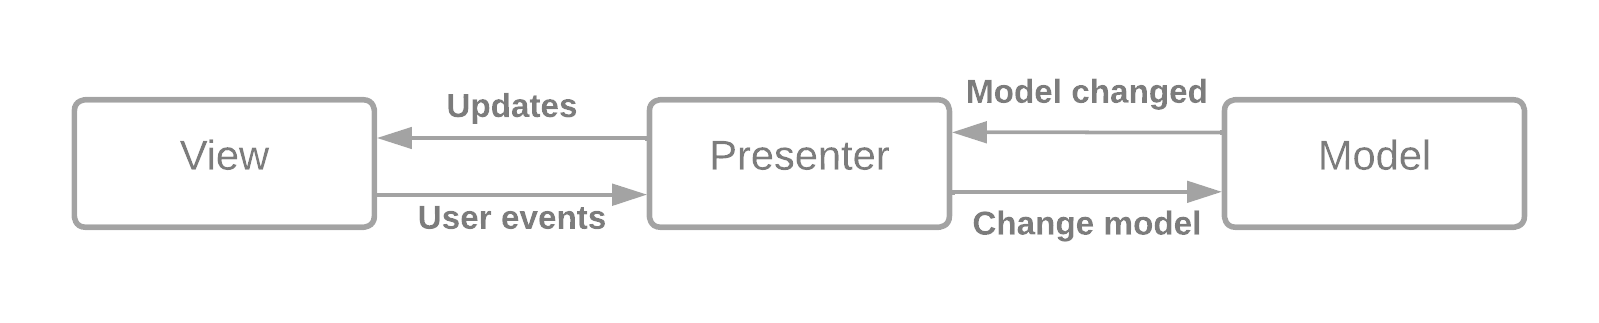
\includegraphics[width=1\textwidth]{./images/MVP.png}
                \caption[Datenfluss in MVP Architektur]{Datenfluss in MVP Architektur \footnotemark}
                \label{fig:MVP}
            \end{figure}
            \footnotetext{Eigene Quelle}



    \subsection{Software Testing}
        \import{./Sections/Introduction/SoftwareTesting}{SoftwareTesting}

        \subsubsection{Testing Pyramide}
            \import{./Sections/Introduction/SoftwareTesting/sub/}{TestingPyramide}
        
        \subsubsection{Unit Tests}
            \import{./Sections/Introduction/SoftwareTesting/sub/}{UnitTests}
        
        \subsubsection{Integration Tests}
            \import{./Sections/Introduction/SoftwareTesting/sub/}{IntegrationTests}

        \subsubsection{SystemTests}
            \import{./Sections/Introduction/SoftwareTesting/sub/}{SystemTests}

        \subsubsection{UI Tests}
            \import{./Sections/Introduction/SoftwareTesting/sub/}{uitests}

        \subsubsection{Manual Tests}
            \import{./Sections/Introduction/SoftwareTesting/sub/}{ManualTests}

    \subsection{SOLID}
        \import{./Sections/Introduction/SOLID/}{SOLID}

        \subsubsection{single-responsibility principle}
            \import{./Sections/Introduction/SOLID/sub/}{SingleResponsibilityPrinciple}
        
        \subsubsection{open–closed principle}
            \import{./Sections/Introduction/SOLID/sub/}{OpenClosedPrinciple}
        
        \subsubsection{Liskov substitution principle}
            \import{./Sections/Introduction/SOLID/sub/}{LiskovSubstitutionPrinciple}
        
        \subsubsection{interface segregation principle}
            \import{./Sections/Introduction/SOLID/sub/}{InterfaceSegregationPrinciple}
        
        \subsubsection{dependency inversion principle}
            \import{./Sections/Introduction/SOLID/sub/}{DependencyInversionPrinciple}

    \subsection{GRASP}
        \import{./Sections/Introduction/GRASP/}{GRASP}

    \subsection{OOP Principles}
        \import{./Sections/Introduction/OOPPrinciples/}{OOPPrinciples}

        \subsubsection{Abstraction}
            \import{./Sections/Introduction/OOPPrinciples/sub}{Abstraction}

        \subsubsection{Encapsulation}
            \import{./Sections/Introduction/OOPPrinciples/sub}{Encapsulation}

        \subsubsection{Inheritance}
            \import{./Sections/Introduction/OOPPrinciples/sub}{Inheritance}

        \subsubsection{Polymorphism}
            \import{./Sections/Introduction/OOPPrinciples/sub}{Polymorphism}

\newpage

\section{Software Architektur}
    \subsection{Was ist eine Software Architektur}

    Bevor man anfängt über die Software Architektur zu reden, muss man sie erstmal definieren.
    Es gibt keine einheitliche Definition einer Software Architektur. Verschiedene Authoren definieren es auch unterschiedlich.

    Robert Martin definiert es als ein Gegenstand mit bestimmten Eigenschaften zu definieren.\\
    \textit{Softwarearchitektur ist die Gestalt des Systems erstellt von derjenigen, die das entwickeln. 
    Die Form dieser Gestalt ist das Aufteilen des Systems in Komponenten, die Anordnung (Arrangement) dieser Komponenten und die Wege, 
    wie diese Komponente miteinander kommunizieren} \cite[136]{cleanArchitecture}
    
    Ralph Jonson definiert Software Architektur aus Sicht eines Projektes.\\
    \textit{Architektur besteht aus den Entscheidungen, die man sich wünscht so früh wie möglich in einem Projekt zu treffen}
    \cite{MF_WhatIsSA}

    In dem ersten Teil des Kapitels wird die Softwarearchitektur aus Sicht eines Projektes betrachtet, 
    indem es kurz beschrieben wird, welche Auswirkungen eine gute und eine schlechte Architektur auf ein Projekt haben kann.

    In dem 2. Teil des Kapitels, wird die Architektur des OCPP Backend Servers beschrieben
    \begin{itemize}
        \item Aufteilung des Programms in einzelne Teile
        \item Testbarkeit und Erweitbarkeit einzelner Teile des Programms
        \item Kommunikation zwischen den einzelnen Teilen
    \end{itemize}

    \subsection{Ziele der Software Architektur}

    Jede Software erfüllt bestimmte Anforderungen, die von Außen gestellt werden. 
    Diese Anforderungen sind meistens von nicht Softwareentwicklern definiert und beziehen sich auf nicht Informatikgebiete 
    (z.B. Banksoftware oder ein Smartphone Anwendung). 
    Das Erfüllen von diesen Anforderungen ist das Ziel von jedem Softwareprojekt.
    Jedoch bei der Umsetzung entstehen viele Herausforderungen, die für die Außenstehenden nicht bekannt sind 
    (z.B. Auswahl einer Datenbank oder Optimierung der Ressourcenverwendung). 

    \textbf{fehlt gluetext}

    \textit{Das Ziel der Software Architektur ist das Mininimieren der menschlichen Ressourcen, 
    die benötigt werden um ein System zu entwickeln und zu unterstützen.}\cite[5]{cleanArchitecture}

    Diese Aussage lässt sich sehr einfach überprüfen, indem man feststellt, 
    ob jede neue Anforderungen an der Software mehr Ressourcen verbraucht als die vorherigen.

    \textit{Das Ziel der Softwarearchitektur ist so viel Entscheidungen wie möglich so spät wie möglich zu treffen}
    \cite[136]{cleanArchitecture}

    Beispiele für solche Entscheidungen wären:
    \begin{itemize}
        \item Datenbanksystem
        \item Transferprotokoll zu der Benutzeroberfläche (z.B. HTTP oder WS) falls vorhanden
        \item Wie und wo die Loggingdaten gespeichert werden (in einer Datei, Datenbank oder externe Server)
    \end{itemize}

    Auch die Tätigkeiten, die nicht mit Programmieren direkt zu tun haben, werden von den Entscheidungen in der Softwarearchitektur betroffen
    \begin{itemize}
        \item Deployment (Aufsetzung) der Software.
        \item Maintenance (Unterstützung) der Software.
    \end{itemize}

    Deployment der Software beinhaltet die Kosten die durch das Aufsetzen der neuen Version der Software entstehen.\\
    Maintenance der Software beinhaltet die Kosten, die nach dem Beenden der Entwicklung bei kleineren Erweiterungen und Änderungen des Systems entstehen.


    \subsection{Technische Schulden}
    Bei den Änderungen oder Erweiterungen eines Systems oft entsteht ein Overhead, das durch die ``Unsaubarkeit'' des bestehenden Programms verusacht wird.

    Dieses Overhead wird als technische Schulden (en. : Technical Debts) bezeichnet.

    Die technischen Schulden entstehen dadurch, dass bei der Entwicklung eines Teiles des Systems wurde 
    von den Entwicklungsteam weniger Zeit investiert um die nicht gewinnbringende Aufgaben zu erledigen.
    Beispiele für solche Tätigkeiten wären:
    \begin{itemize}
        \item Unittests
        \item Dokumentieren 
        \item Code Review
    \end{itemize}

    Beispiele für Technische Schulden wären:
    \begin{itemize}
        \item Alte Funktionalitäten funktionieren nach der Änderung nicht mehr
        \item Aufdeckung eines Bugs erst nach einer gewissen Zeit in Produktionsversion der Software
        \item Implementieren der neuen Funktionalitäten verbraucht deutlich mehr Zeit
    \end{itemize}

    Eine klare Struktur der Software reduziert die Menge an technischen Schulden, 
    die die Weiterentwicklung in der Zukunft verlangsamen. 

    Die Softwareentwickler können die ankommenden Aufgaben erledigen
    \begin{itemize}
        \item man hat bereits Vorgaben wie die Kommunikationswege zwischen den Modulen ist
        \item wie die Module benannt werden sollen
        \item an welchen Stellen das Modul in das System hinzugefügt werden soll
        \item die Menge an durch den "Zufall" entstehenden Bugs in anderen Teilen des Programms ist minimal
    \end{itemize}

    Durch die bereits definierten Kommunikationswege zwischen den Modulen, muss weniger Dokumentation geschrieben werden.
    Mit weniger Dokumentation findet man schneller die gesuchten Informationen.

    Durch die einheitliche Bezeichnung der Teile des Modules kann man allein aus dem Namen des Modules seine Aufgaben ableiten.

    Daher ist es vom Vorteil bevor man mit der Umsetzung des Softwaresystems anfängt, die oben gennanten Aufgaben zu lösen,
    denn mit zunehmender Lebenszeit der Software nimmt die Änderungszeit zu.

    Somit lassen sich die vorhandenen Ressourcen effizienter eingesetzen.

    \newpage
    \subsection{Qualität und Kosten der Software}
    \nocite{MF_isHighQuilatySoftwareWorthTheCost}

    Am Anfang jedes neuen Projektes in der Softwareentwicklung muss die Entscheidung getroffen werden, wie qualitativ gut die Software am Ende sein soll.
    Damit sind die Eigenschaften/Funktionalitäten der Software gemeint, die für die Benutzer irrelevant sind, jedoch eine sehr große Bedeutung 
    für das Entwicklungsteam haben.
    
    Wenn man eine qualitativ gute Software hat, ergeben sich unteranderem folgende Vorteile:
    \begin{itemize}
        \item Bugs können schneller lokalisiert und beseitigt werden
        \item Neue Funktionalitäten können mit weniger Aufwand umgesetzt werden
        \item Die Änderungen der Funktionalitäten können schneller umgesetzt werden
        \item Die Wahrscheinlichkeit bestehende Funktionalitäten ungewollt zu ändern veringert sich
        \item Die Einarbeitungszeit von neuen Teammitgliedern verkürzt sich 
    \end{itemize}

    Alle diese Vorteile hat man nicht kostenlos, denn dafür muss man auch Zeit investieren indem man:
    \begin{itemize}
        \item Regelmäßig die Software refactored
        \item Code Qualität überprüft
        \item Code Reviews durchführt
        \item Automatisierte Tests schreibt (Unit-, Integration- und Systemtests)
        \item Dokumentation aktuell hält
        \item Die technischen Schulden gering hält
    \end{itemize}

    Nicht in jedem Projekt ist das Umsetzen von oben genannten Eigenschaften möglich, 
    denn man hat nicht genug Zeit oder das Budget ist zu klein dafür.
    Man kann aber gewisse Kriterien setzen um mit deren Hilfe bessere Entscheidung zu treffen:
    \begin{itemize}
        \item Wann soll die MVP\footnote[1]{Minimum viable product} vorhanden sein.
        \item Wie viele Ressourcen man zur Verfügung hat
        \item Wie wahrescheinlich sind die Änderungen und Erweiterungen der Software
        \item Wie kritisch verschiede Probleme und Ausfälle der Software sind 
    \end{itemize}

    Auf dem unterer Darstellung sieht man, dass auf langere Distanz eine gute Softwarearchitektur deutlich
    mehr Funktionalitäten besitzt als eine Software mit schlechter Architektur. 
    Jedoch es gibt einen Zeitinterval, in dem die schlectere Software besser da steht.
    \begin{figure}[H]
        \centering
        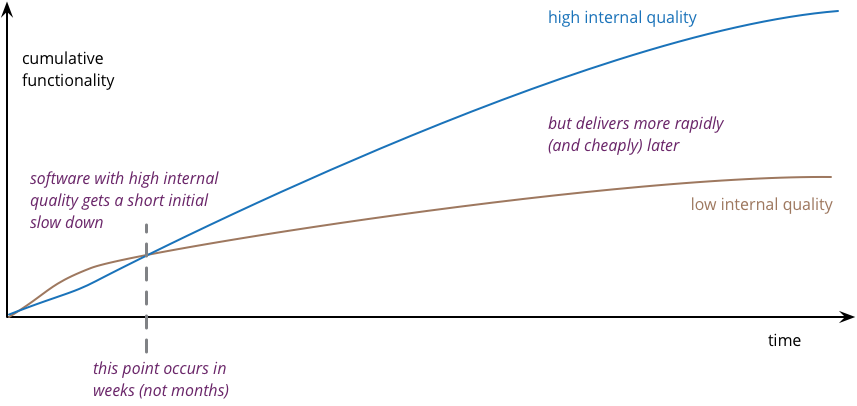
\includegraphics[width=1\textwidth]{./images/QASoftwareCompare.png}
        \caption[Vergleich einer guten und einer schlechten Softwarearchitektur]{Vergleich einer guten und einer schlechten Softwarearchitektur \footnotemark}
        \label{fig:softQuality}
    \end{figure}
    \footnotetext{https://martinfowler.com/articles/is-quality-worth-cost.html}
    Diese Eigenschaft muss man immer beim Projektbegin beachten, denn es wäre Zeitaufwändig für ein Studiumprojekt, 
    für das man evtl. nur eine Woche Zeit hat, um eine komplexe Architektur zu implementieren, die ohne jeglichen Funktionalitäten mehrere Wochen gebrauchen wird.

    Wenn man aber ein Projekt hat, das regelmäßig weiterentwickeln wird, ist es vom Vorteil gleich eine gute Architektur umzusetzen.

    \subsection{Wichtigkeit der Testbarkeit der Software}
    Jedes Teil der Software wird in seinem Lebenszyklus mehrmals geändert. 
    Um die Funktionalität der neuen Version zu verifizieren, muss sie getestet werden.
    Es ist von Interesse diese Aufgabe zu automatisieren. 
    Wie in den früheren Kapitels bereits beschrieben wurde, am schnellsten findet man die Bugs, falls vorhanden, mit Unittests. 
    Bei den Unittests müssen die Module (z.B. einzelne Klassen in Falle von OOP Sprachen) in verschiedenen Umgebungen überprüft werden. 
    Das heißt, dass die Zustände von benutzten Modulen müssen einfach zu simulieren sein.
    Dies erfordert eine Planung der Softwarearchitektur im Voraus, 
    um diese Eigenschaft zu implementieren um im Laufe der Entwicklung, Zeit durch automatisierte Tests zu sparen.

    \newpage
    \subsection{Technische Umsetzung der Software Architektur}

    Der OCPP Backend Server wurde anhand ``Clean Architecture'' projektiert und entsprechend umgesetzt. 
    Im Kapitel werden die benutzten Schichten beschrieben, welche Eigenschaften sie besitzen und wie sie miteinander verbunden sind.
    Auch wird kurz gezeigt wie es mit der Testbarkeit auf allen Niveaus (Unit, Integration und Systemtests), 
    Änderbarkeit und Erweitbarkeit der Software ist.

    \import{./images/}{circle_1}
    \footnotetext{Eigene Quelle}

    Beschreibung der Darstellung:
    Jede Komponente bringt in das gesamt Programm folgende Teile:
    \begin{itemize}
        \item Port - z.B. WebSocket Server aufzubauen
        \item Adapter  - umwandeln der ankommenden Nachrichten bzw. Ereignisse in die Typen definierten im Domain
        \item Controller - definiert alle Tätigkeiten, die die Komponente machen könnte
        \item UseCase - definiert den Ablauf an Tätigkeiten (Interactoren) beim Geschehen eines Ereignisses
        \item Interactors - Hülle für alle definierten Tätigkeiten im Controller
        \item Domain - definiert Typen benutzten der Komponente und deren Basic Verhalten, auch die Ereignisse die vom Dispatcher verteilt werden
    \end{itemize}

    \newpage
    \subsection{Abhängigkeiten im Programm}
    \label{kap:Structur}

    Die Architektur lässt sich in zwei wesentlichen Teilen zerlegen
    \begin{itemize}
        \item Anbindung an Infrastruktur um das Programm (Port - Adapter - Controller)
        \item Innere Logik des Programms (Controller - Dispatcher - UseCase - Interactor)
    \end{itemize}

    Beispiele für die Infrastruktur sind: Datenbank, Persistenz, Schnittstellen (HTTP, USB usw)

    Bei solcher Aufteilung ergeben sich folgende Vorteile:
    \begin{itemize}
        \item Innere Logik des Programms lässt sich mittels Integrationstests unabhängig von Schnittstellen abdecken.
        Damit ist die Laufzeit von jedem einzelnen Test ohne reelen Schnittstellen ist schneller als mit reelen Schnittstellen und 
        man hat das gleiche Ergebnis bezüglich des Verhaltens des Programms.
        \item Die Innere Logik ist nicht an Schnittstellen gebunden, 
        somit können alle Schnittstellen mit wenig Aufwand getauscht werden.
    \end{itemize}

    \subsubsection{Port-Adapter-Controller}
    \label{Port-Adapter-Controller}
    Am nähesten zu der \textbf{PAC}\footnote{Port-Adapter-Controller} Struktrur 
    ist das Pattern \textbf{MVP}\footnote{Model-View-Presenter}.
    Dabei die Aufgaben von \textbf{View} entsprechen den Aufgaben von \textbf{Port}. 
    Die Aufgaben von \textbf{Presenter} entsprechen den Aufgaben \textbf{Adapter}.
    Und die Aufgaben von dem Rest des Programms inklusiv \textbf{Controller} entspechen den Aufgaben von \textbf{Model}.

    Der Unterschied zu \textbf{MVP} besteht darin, dass \textbf{MVP} im klassischen Sinne nur für die Benutzerobeflächen gedacht ist,
    während in der hier beschriebenen Umsetzung wird es für alle Schnittstellen benutzt.
    \textbf{MVP} Architektur übernimmt in der gesamten Application eine zentralle Stelle und ist nur einmal zu treffen.
    \textbf{PAC} ist nur ein Teil der gesamten Application, wird an mehreren Stellen unterschiedlich benutzt und beschreibt nicht 
    die Architektur der Application.


    \begin{figure}[H]
       \centering
       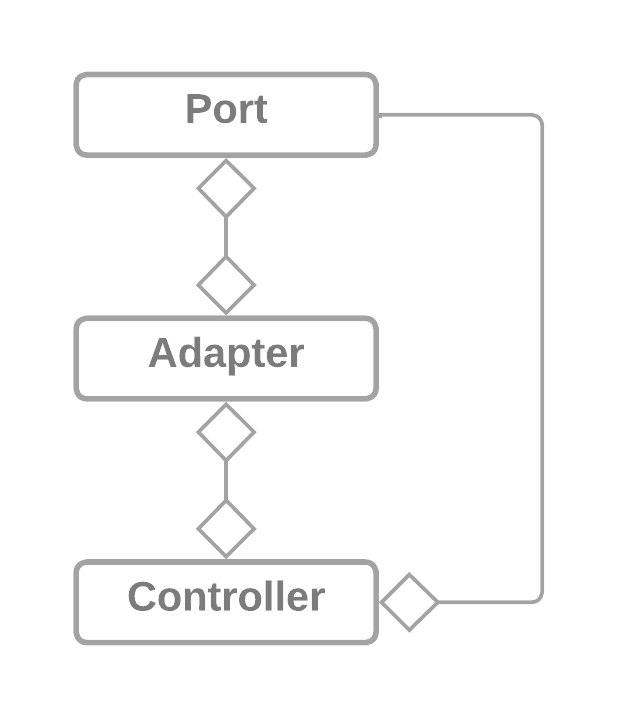
\includegraphics[width=6.5cm]{./images/Port-Adapter-Contoller.png}
        \caption[Objektendiagramm PAC]{Objektendiagramm PAC \footnotemark}
        \label{fig:CDPAC}
    \end{figure}
    \footnotetext{Eigene Quelle}

    \subsubsection{Controller-Dispatcher-UseCase-Interactor} 
    \label{Controller-Dispatcher-UseCase-Interactor}
    In dem Teil wird die komplete innere Logik der Application beschrieben. Dafür ist nur \textbf{Controller} notwendig. 
    D.h. beim Geschehen eines Ereignisses wird eine (oder mehrere) Method(en) in deb jeweiligen Controllern aufgerufen,
    die das Ereignis entsprechend abarbeiten.
    Dabei hat man folgendes Problem:
    jeder \textbf{Controller} übernimmt mehrere Aufgaben 
    (z.B. Kontrollieren von \textbf{Port} und \textbf{Adapter} und enthält Anwendungslogik)
    d.h. keine \textbf{SRP}

    Eine mögliche Lösung wäre das Separieren von Kontrollieren von \textbf{Port} und \textbf{Adapter} und Anwendungslogik
    in 2 verschiedenen Teile. Die Anwendungslogik heißt \textbf{UseCase}.

    Bei dieser Aufteilung besteht das Problem, dass beim Geschehen eines Ereignisses im \textbf{Controller} muss dieses Ereignis an das 
    richtige \textbf{UseCase} zugeordnet werden. D.h. \textbf{Contoller} besitzt eine weitere Verantwortlichkeit die sich in ein anderes Teil
    verschieben lässt. Dieses Teil heißt \textbf{Dispatcher}, dessen Aufgabe ist das Informieren alle daran Interessierten \textbf{UseCase}s
    beim Geschehen eines Ereignisses. 

    Jedes \textbf{UseCase} kann mehrere aufeinander folgende Aufgaben machen.
    Alle Aufgaben müssen gleiche Funktionalitäten besitzen, z.B:
    \begin{itemize}
        \item der Anfang und das Ende in Logs aufzeichnen.
        \item Nach einer bestimmten Zeit gestoppt werden.
    \end{itemize}
    D.h. man braucht eine ``Hülle'' um jeder Methode - \textbf{Interactor}

    Wenn man das alles zusammen entsteht folgendes Objektendiagramm:

    \begin{figure}[H]
        \centering
        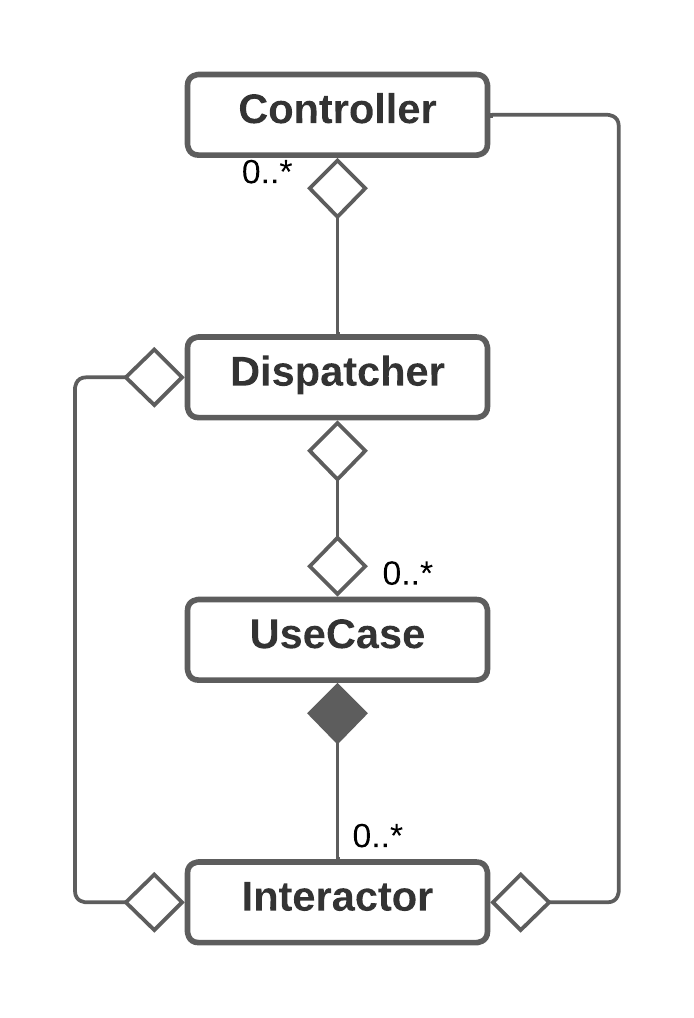
\includegraphics[width=6.5cm]{./images/Controller-Dispatcher-UseCase-Interactor.png}
         \caption[Objektendiagramm Controller-Dispatcher-UseCase-Interactor]{Objektendiagramm Controller-Dispatcher-UseCase-Interactor \footnotemark}
         \label{fig:CDCDUI}
    \end{figure}
    \footnotetext{Eigene Quelle}

    \newpage
    \subsubsection{Erstellen der Struktur}
    In den Kapiteln \ref{Controller-Dispatcher-UseCase-Interactor} und \ref{Port-Adapter-Controller} 
    werden die fertigen Strukturen beschrieben, diese Strukturen müssen am Anfang des Programms erstellt
    und miteinander verbunden werden.

    Das Erstellen von der Struktur findet im \textbf{Main} statt und lässt sich in drei Schritte aufteilen:
    \begin{itemize}
        \item Erstellen alle Instanzen
        \item Verknüpfen alle Instanzen miteinander
        \item Starten alle Instanzen
    \end{itemize}

    Das Erstellen aller Instanzen lässt sich in zwei weitere Schritte aufteilen, die bedingt voneinander abhängen.
    \begin{itemize}
        \item Core (Controllers + Dispatcher + UseCases + Interactors)
        \item Schnittstellen (Port + Adapter + Controller)
    \end{itemize}

    Damit auch Integrationstests für den kompleten Core und jede Schnittstellen möglich sind, wäre es sinnvol, dass beide Schritte
    explicit ausgeführt werden.

    Ein möglicher Ablauf wäre:
    \begin{figure}[H]
        \centering
        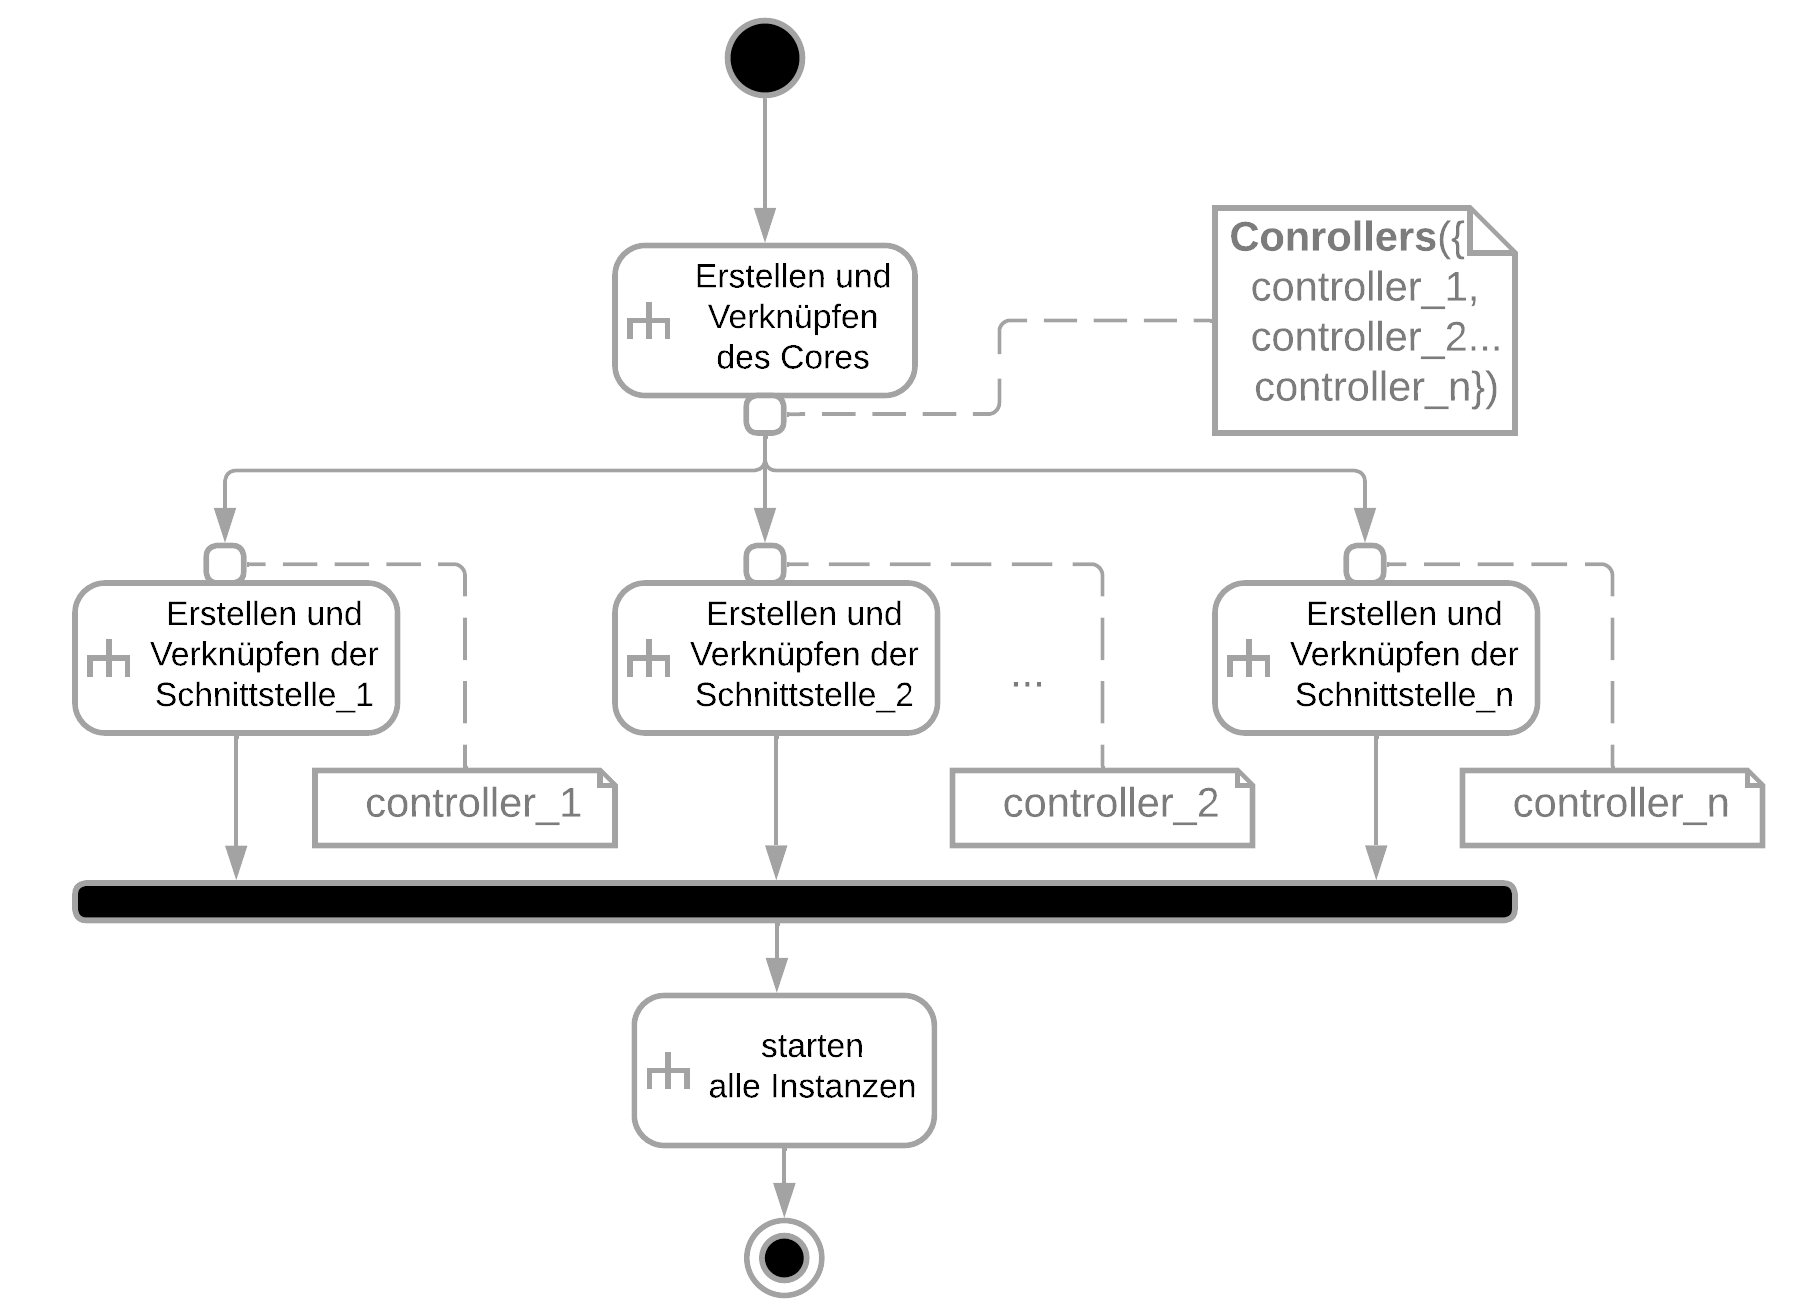
\includegraphics[width=12cm]{./images/Erstellen AD.png}
         \caption[Ablaufiagramm Erstellen der Struktur]{Ablaufiagramm Erstellen der Struktur \footnotemark}
         \label{fig:ADCreate}
    \end{figure}
    \footnotetext{Eigene Quelle}

    Mit diesem Ablauf können mehrere \textbf{Main}s erstellt werden, die verschiedene Anwendungen für verschiedene Zwecke erstellen.
    Z.B. ein Framework braucht keine reelen Anknüpfungen an die Infrastruktur (z.B. Datenbank) im Vergleich zu Standalone Anwendung.
    Oder es können verschiedene \textbf{Main}s für verschiedene Datenbanken.

    \subsubsection{Utility Controllers}
    \label{kap:utilityControllers}
    In jeder Anwendung gibt es Teile bzw. Module, die aus allen Orten erreichbar sein sollen
    (z.B. Logger Controller oder Datum Controller), und es gibt auch Klassen, die regelmäßig instanziert werden.

    Das Problem dabei ist, dass in das neue erstellte Objekt die Utility Controllers immer neben den anderen Argumenten 
    mitübergeben werden müssen. Das erschwert die Lesbarkeit des Codes und kann eine Reihe an Änderungen an vielen Stellen mit sich ziehen,
    falls man die Konstruktoren ändert.
    
    Es gibt folgende Möglichkeiten das Problem zu lösen:
    \begin{itemize}
        \item Globale Objekte bzw. Instanzen (z.B. OOP Design Pattern \textbf{Singleton} \ref{kap:gof:singleton})
        \item Initialisiereung von den Entsprechenden Instanzen und Übergeben in dem Konstruktor (OOP Sprachen)
        oder mittels einer Settermethode.
    \end{itemize}

    Bei der ersten Implementierung hat man das Problem, dass die benutzten Utility Controllers nicht ersetzbar sind.
    D.h. man kann dann alle Module sehr schwer mit Unittests abdecken, denn es werden immer auch die Utility Controllers mitgetestet.
    Ein weiteres Problem besteht darin, dass alle Utility Controllers eine Infrastruktur benutzen.
    (z.B. Logs in dem Datenbank speichern). Jeder Test wird dadurch deutlich länger laufen, als es sein könnte.
    Da es auch reele Infrastruktur sein wird, wird es die Parallelisierung des Tests deutlich erschwert, denn 
    der Zustand der benutzten Infrastruktur durch mehrere unabhängig voneinander laufendenen Tests geändert wird.

    Bei der zweiten Möglichkeit müssen alle Utility Controllers entweder bei der Initialisiereung im Konstruktor 
    der jeweiligen Instanzen übergeben, dies führt zu einer längeren Parameterliste,
    die die Lesbarkeit des Codes erschwert oder mittels einer Settermethode der Instanz,
    dies führt dazu, dass der Aufruf der Methode von dem Softwareentwickler vergessen werden kann.
    
    Das Problem lässt sich zum Beispiel durch OOP design pattern \textbf{Factory}, das die Utility Controllers bereits
    enthält und bei der Initialisiereung entsprechend in Konstruktor übergibt. 
    Jedes Teil des Programms besitzt eine Referenz auf der Instanz der Fabrik, 
    die eine kürzere Interface für das erstellen von verschieden Instanzen anbietet.
    Alle Module bzw. Klassen lassen sich somit auch mit Unittests
    abdecken, da die Utility Controllers entsprechend gemockt werden können. 

    In der Abbildung \ref{fig:CDControllerWithUtility} ist die Verbindung jedes \textbf{Controller}s mit den Utility Controllers als Klassendiagramm dargestellt.
        
    \begin{figure}[H]
        \centering
        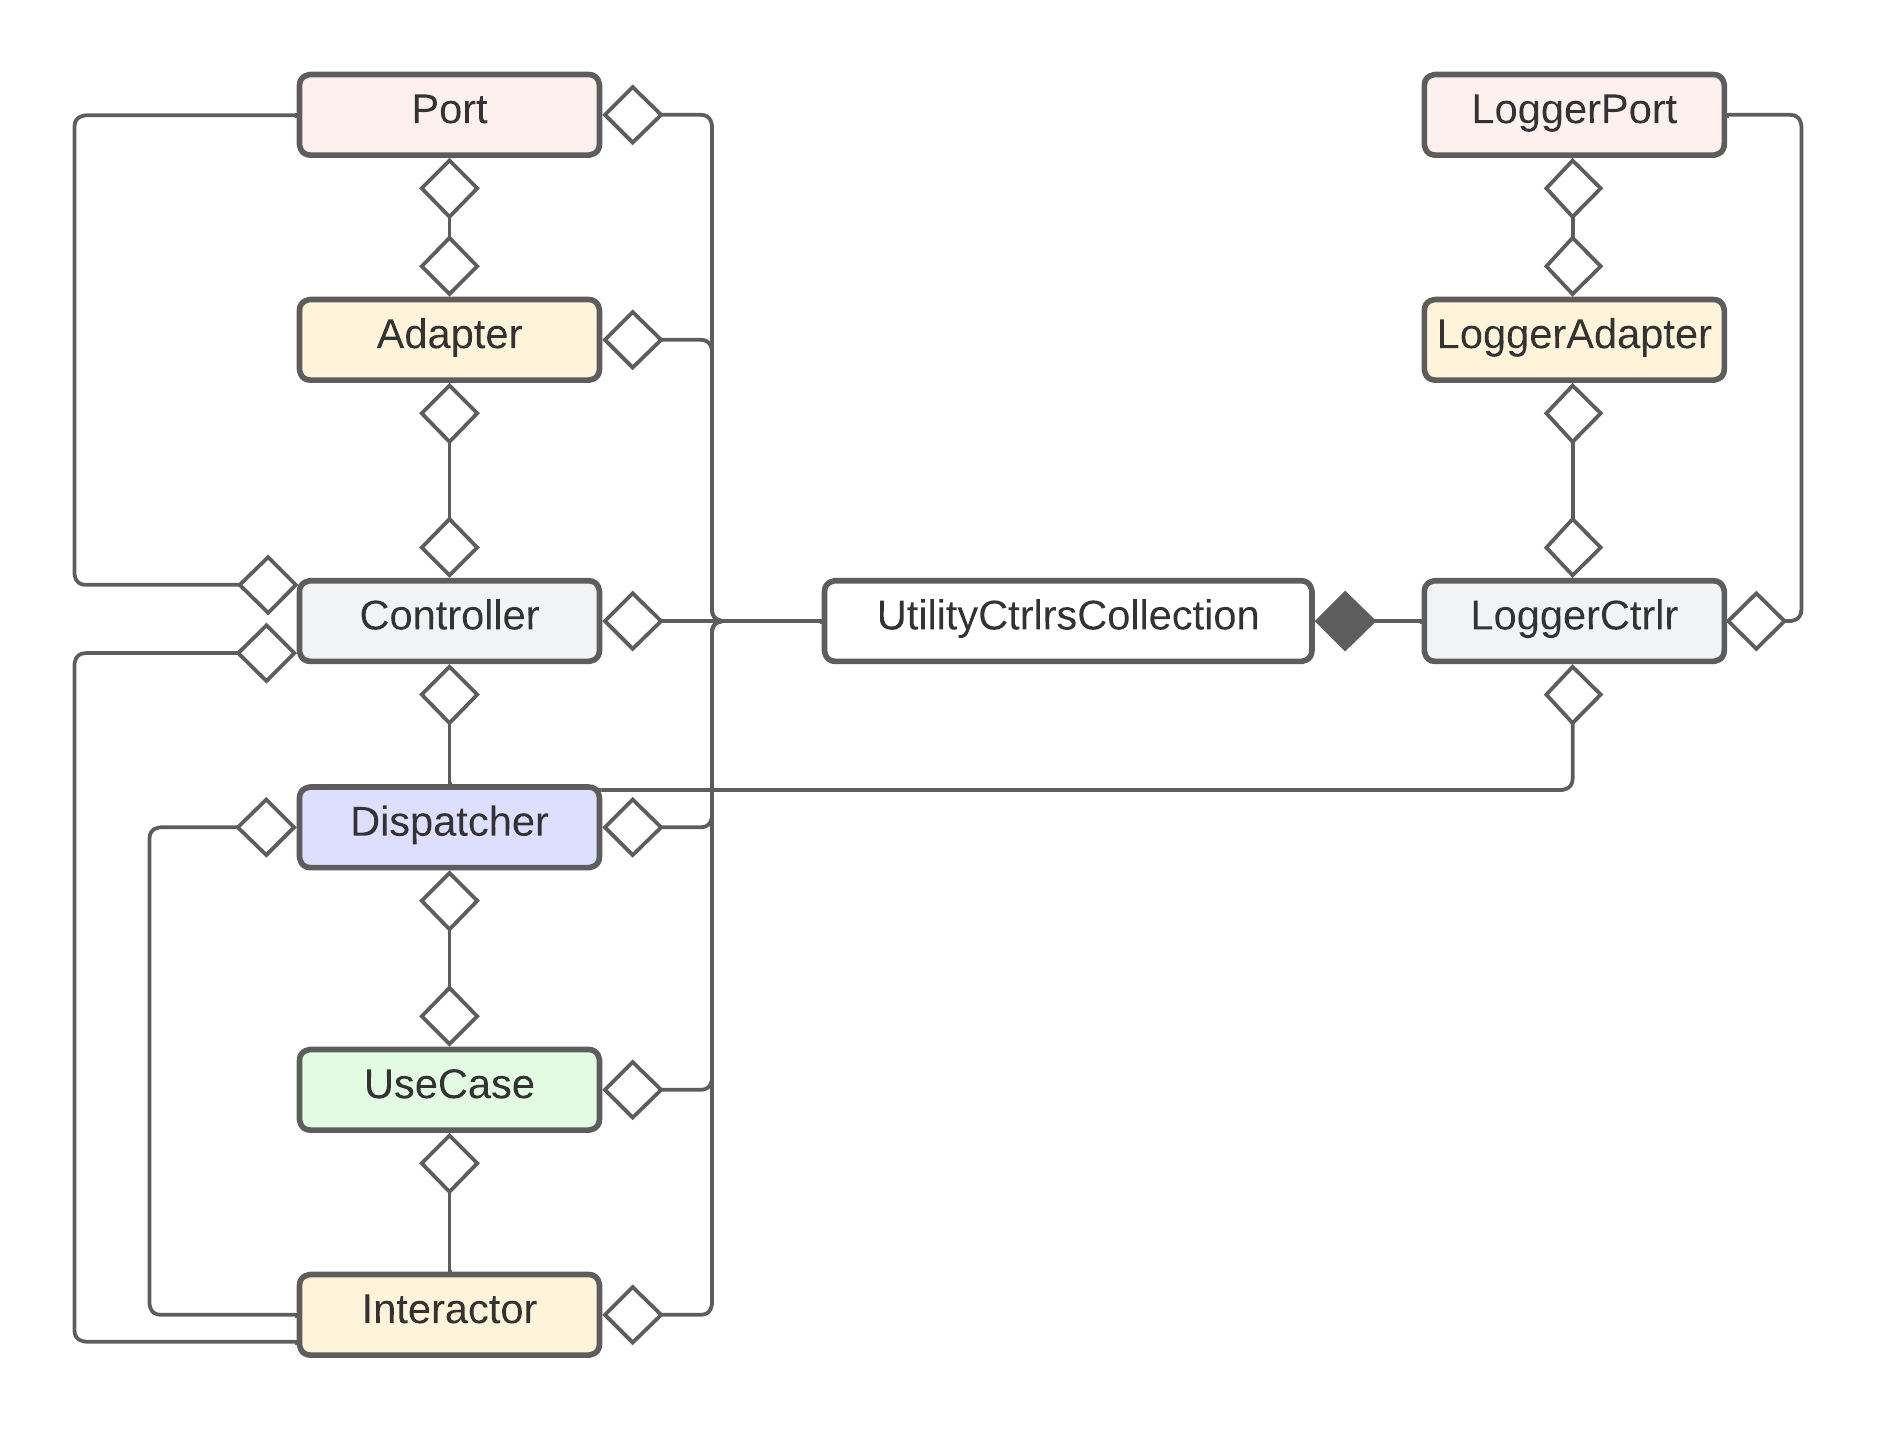
\includegraphics[width=12cm]{./images/KlassendiagramMitUtilityControllers.png}
         \caption[Objektendiagramm mit Utility Controllers]{Objektendiagramm mit Utility Controllers \footnotemark}
         \label{fig:CDControllerWithUtility}
    \end{figure}
    \footnotetext{Eigene Quelle}

    \subsubsection{Verbindung der einzelnen Schichten miteinander und die Testbarkeit}
    Die früheren Kapitels beschreiben mittels Objektendiagramms die Struktur der Anwendungen nach dem Starten.

    Die Schichten sind mittels \textbf{\nameref{DependencyInjection}} miteinander verknüpft.

    Beispiel für \textbf{Port}-\textbf{Adapter}-\textbf{Controller} Verbindung:

    \begin{figure}[H]
        \centering
        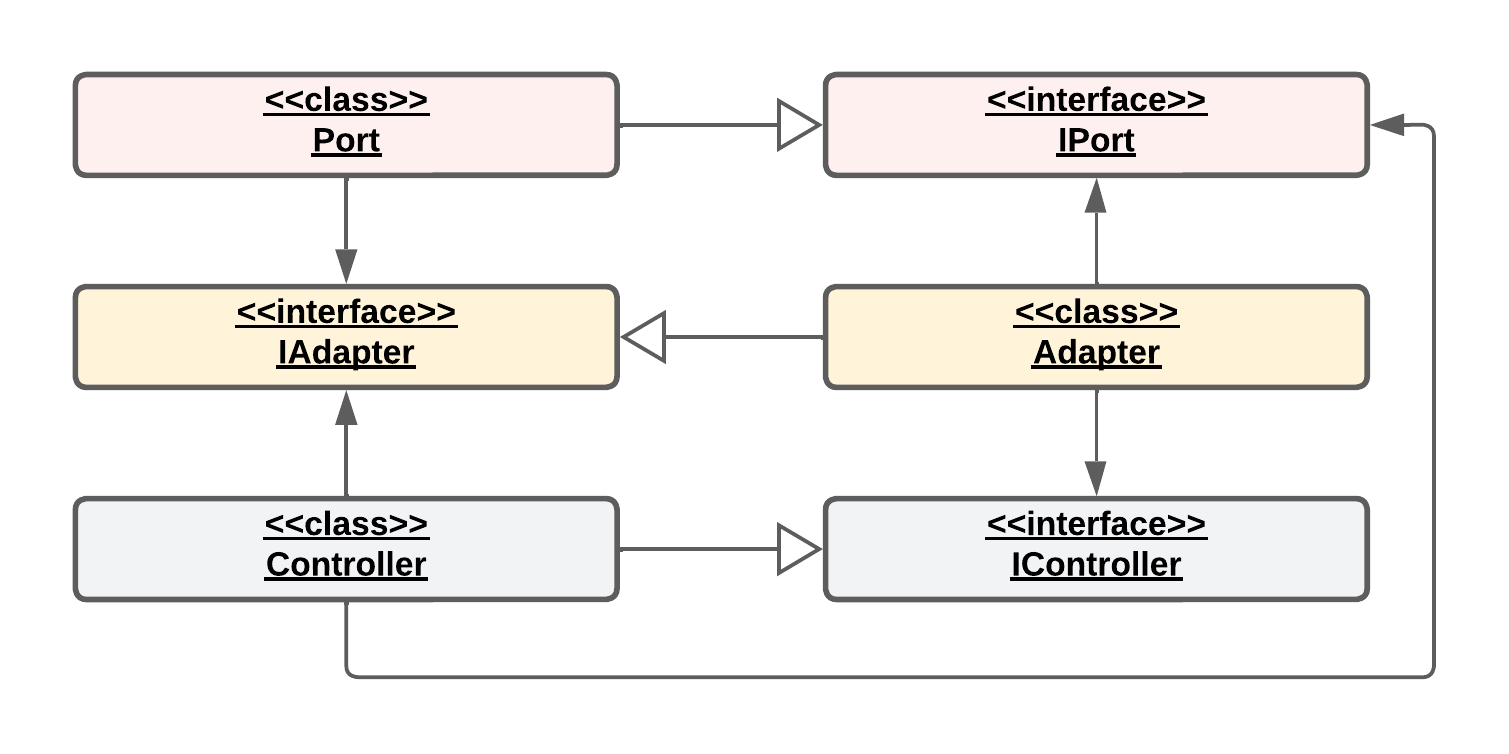
\includegraphics[width=12cm]{./images/Klassendiagramm Port-Adapter.png}
        \caption[Klassendiagramm Port-Adapter-Controller]{Klassendiagramm Port-Adapter-Controller \footnotemark}
        \label{fig:FullCDPAC}
    \end{figure}
    \footnotetext{Eigene Quelle}

    Im Klassendiagramm \ref{fig:FullCDPAC} sind alle Klassen miteinander über ein Interface verbunden.
    Dies ermöglicht leichte und schnelle Ersetzbarkeit der Schichten und 
    somit lässt sich jeder Zustand der Umgebung um einer Schicht simulieren. 
    Das ist Voraussetzung für Testbarkeit jeder einzelnen Schicht unabhängig von den anderen Schichten.

    \newpage
    \subsection{Datenfluss im Programm}
    \label{kap:Dataflow}
    Im System gibt es 3 wichtige Datenflusse, die durch Kombination miteinander die komplexen Abläufe im System umsetzen
    \begin{enumerate}
        \item (blau) Controller löst ein Ereignis im Dispatcher aus.
        \item (rot) Controller spricht sein Port an(z.B. Speichern der Daten in der Datenbank oder OCPP Antwort abzuschicken)
        \item (grün) Das Programm wird von einem externen System angesprochen (z.B. Ladesäule schickt eine OCPP Nachricht an den Server) 
    \end{enumerate}
    Wenn das geschehen ist, sieht der Datenfluss so aus:
    \import{./images/}{circle_2}
    \label{fig:sp2d}
    \footnotetext{Eigene Quelle}

    \newpage
    Darstellung des Datenflusses \textbf{1} als \textbf{Sequencediagram}:

    \begin{figure}[h]
        \begin{sequencediagram}
            \newthread{A}{Controller 1}
            \newinst[1]{B}{Dispatcher}
            \newinst[1]{C}{UseCase}
            \newinst[1]{D}{Interactor I}
            \newinst[1]{E}{Controller J}
            
            \begin{messcall}{C}{subscribe ``Event''}{B}
            \end{messcall}

            \begin{messcall}{A}{Event}{B}{}
                    \begin{messcall}{B}{Event}{C}{}
                        \begin{sdblock}{Loop}{Until sequence of use case done}
                            \begin{call}{C}{Handle I}{D}{result}
                                \begin{call}{D}{Handle I}{E}{result}
                                \end{call}
                            \end{call}
                        \end{sdblock}
                    \end{messcall}
            \end{messcall}
          \end{sequencediagram}
          \caption{Sequencediagramm vom Datenfluss ``1'' Blau}
          \label{fig:seqDiagBlue}
    \end{figure}

    Wenn im \textbf{Controller} ein Ereignis erzeugt wird, wird \textbf{Dispatcher} darüber informiert. ein
    oder mehrere \textbf{UseCases} haben bereits dieses Event bei \textbf{Dispatcher} aboniert.
    \textbf{Dispatcher} informiert alle auf das Ereignis abonierte \textbf{UseCases}. 
    Jeder UseCases kann seinen eigenen Verhalten auf das Event definieren unabhängig voneinander.
    \textbf{UseCase} definiert einen Ablauf an \textbf{Interactoren},
    die wie vorgeschrieben ausgeführt werden. Jeder \textbf{Interactor} ruft eine Methode von einem \textbf{Controller} auf 
    und das Ergebnis wird an \textbf{UseCase} zurückgegeben, das vom UseCase entsprechend behandelt wird.

    \newpage
    Dabei es gibt 2 Möglichkeiten wie das Ereignis vom \textbf{Controller J} das \textbf{Interactor I} erreichen kann:
    \begin{enumerate}
        \item synchron - der Rückgabewert ist das Ergebnis der aufgerufenen Methode 
        \item asynchron - man wartet auf dazugehörige Antwort vom Port (z.B. auf OCPP Response warten, wenn man ein OCPP Request abschickt)
    \end{enumerate}

    Darstellung der 2. Möglichkeit:
    \begin{figure}[h]
        \begin{sequencediagram}
            \newthread{U}{UseCase}
            \newinst[1]{A}{Interactor I}
            \newinst[2]{C}{Dispatcher}
            \newinst[1]{B}{Controller J}
            \newthread{D}{...Externe}
            
            \begin{call}{U}{Message}{A}{Response}
            
            \begin{messcall}{A}{Message}{B}{}
                \begin{messcall}{A}{subscribe 'Response'}{C}{}
                    
                \end{messcall}
                \begin{messcall}{B}{Message}{D}{}
                \end{messcall}
            \end{messcall}
            \begin{messcall}{D}{Response}{B}{}
                \begin{messcall}{B}{Response}{C}{}
                    \begin{messcall}{C}{Response}{A}{}

                    \end{messcall}
                \end{messcall}

                \begin{messcall}{A}{unsubscribe 'Response'}{C}{}
                \end{messcall}
            \end{messcall}
            
                
            \end{call}
        \end{sequencediagram}
    \end{figure}

    Der Rückgabewert wird beim synchronen Funktionsaufruf zurückgegeben, wie in der Abbildung ~\ref{fig:seqDiagBlue} dargestellt.
    Der Rückgabewert beim asynchronen Funktionsaufruf, wird wie folgt definiert:
    Der Aufgerufene Interactor ruft eine Methode vom Controller auf, der die Nachricht an den externen Teilnehmer abschickt. 
    Gleich danach abonniert der Interactor die Antwort auf die abgeschickte Nachricht. Wenn die Antwort ankommt, landet sie beim Dispatcher,
    die alle Abonierten darüber informiert, unteranderem auch den Interactor. Der Interactor gibt diese Antwort als Rückgabewert der Funktionsaufruf

    \newpage
    Darstellung des Datenflusses ``2'' als ``sequencediagram'':
    \begin{figure}[h]
        \begin{sequencediagram}
            \newthread{A}{Controller}
            \newinst[1]{B}{Adapter}
            \newinst[1]{C}{Port}
            \newinst[3]{D}{Externe}
            \begin{call}{A}{Message}{B}{return result}
                \begin{call}{B}{Message}{C}{return result}
                    \begin{messcall}{C}{Message}{D}{}
                        
                    \end{messcall}
                \end{call}
            \end{call}
        \end{sequencediagram}
    \end{figure}\\
    Darstellung der Datentransformation:\\
    Controller - Adapter: Alle Informationen werden als Objekte übergeben, die im Domain definiert werden müssen.
    \begin{lstlisting}[language=json,firstnumber=1]
        OCPP20Message({
            destination: {
                chargerId : "some_unique_charger_id"
            },
            message : {
                name : "BootNotification",
                type : "Response",
                payload : BootNotification({
                    currentTime : Date(Thu Jul 28 2022 14:26:49 GMT+0200),
                    interval : 30,
                    status : "Rejected"    
                })
            }
        })
        \end{lstlisting}
        Adapter - Port: Alle Informationen, die gesendet werden (in dem Fall ``message''), werden in der verstandlichen Form (sie muss nicht mehr geändert werden)
        für den Port an Port weitergegeben.
        Über das Ziel müssen alle Informationen weitergegeben werden, so dass Port die entsprechende Verbindung zuordnen kann. 

        \begin{lstlisting}[language=json,firstnumber=1]
        {
            destination : {
                chargerId : "some_unique_charger_id"
            }
            message : "[3, 'message_id_of_request', {currentTime : 'Thu Jul 28 2022 14:26:49Z', interval : 30, status : 'Rejected'}]"
        }
    \end{lstlisting}


    Darstellung des Datenflusses ``3'' als ``sequencediagram'':
    \begin{figure}[H]
        \begin{sequencediagram}
            \newthread{A}{Externe}
            \newthread{B}{Port}
            \newinst{C}{Adapter}
            \newinst{D}{Controller}

            \begin{messcall}{A}{Message}{B}
                \begin{messcall}{B}{Message}{C}
                    \begin{messcall}{C}{Message}{D}
                        
                    \end{messcall}
                \end{messcall}
            \end{messcall}
        \end{sequencediagram}
    \end{figure}
    
    \newpage
    \newpage
    \newpage
    \subsubsection{Logging}
    Ein wichtiger Bestandteil jeder Software ist das Logging von unterschiedlichen Ereignissen in der Software.
    Das Ziel vom Logging ist später von den Softwareentwicklern verschiede Fehler in der Software so schnell wie möglich zu finden und
    zu beseitigen.
    
    Dafür muss es möglich sein mit den Logs die Fehler so genau wie möglich in der Software zu lokalisieren 
    (welche Komponente oder welche Methode den Fehler hervorgerufen hat) 
    und welche Ereigniskette den jeweiligen Fehler hervorgerufen hat.

    In dem Kapitel \ref{kap:Dataflow} sind alle möglichen Wege basierend auf der beschriebenen Struktur 
    im Kapitel \ref{kap:Structur} für die ankommenden Ereignissen in der Software beschrieben.

    Die untere Abbildung \ref{fig:FullDataFlow} zeigt den kompleten Ablauf beim Geschehen eines Ereignisses.
    Eine mögliche Systematisierung des Loggierens in der Appliaction wäre: 
    \begin{itemize}
        \item man zeichnet in jeder Komponente den Inhalt des ankommenden Ereignisses auf
        \item man zeichnet in jeder Komponente den Inhalt des ausgehenden Ereignisses auf
        \item man zeichnet alle Komponenten auf, an die das Ereignis weitergegeben wird
    \end{itemize}

    Somit lässen sich die Fehler auf die Komponente genau lokalisieren, d.h. man kann einen entsprechenden Unittest schreiben, 
    der diesen Fehler abdeckt, bzw. einen Integrationtests, da man auch den Ablauf des Ereignisses kennt.
    
    \begin{figure}[H]
        \centering
        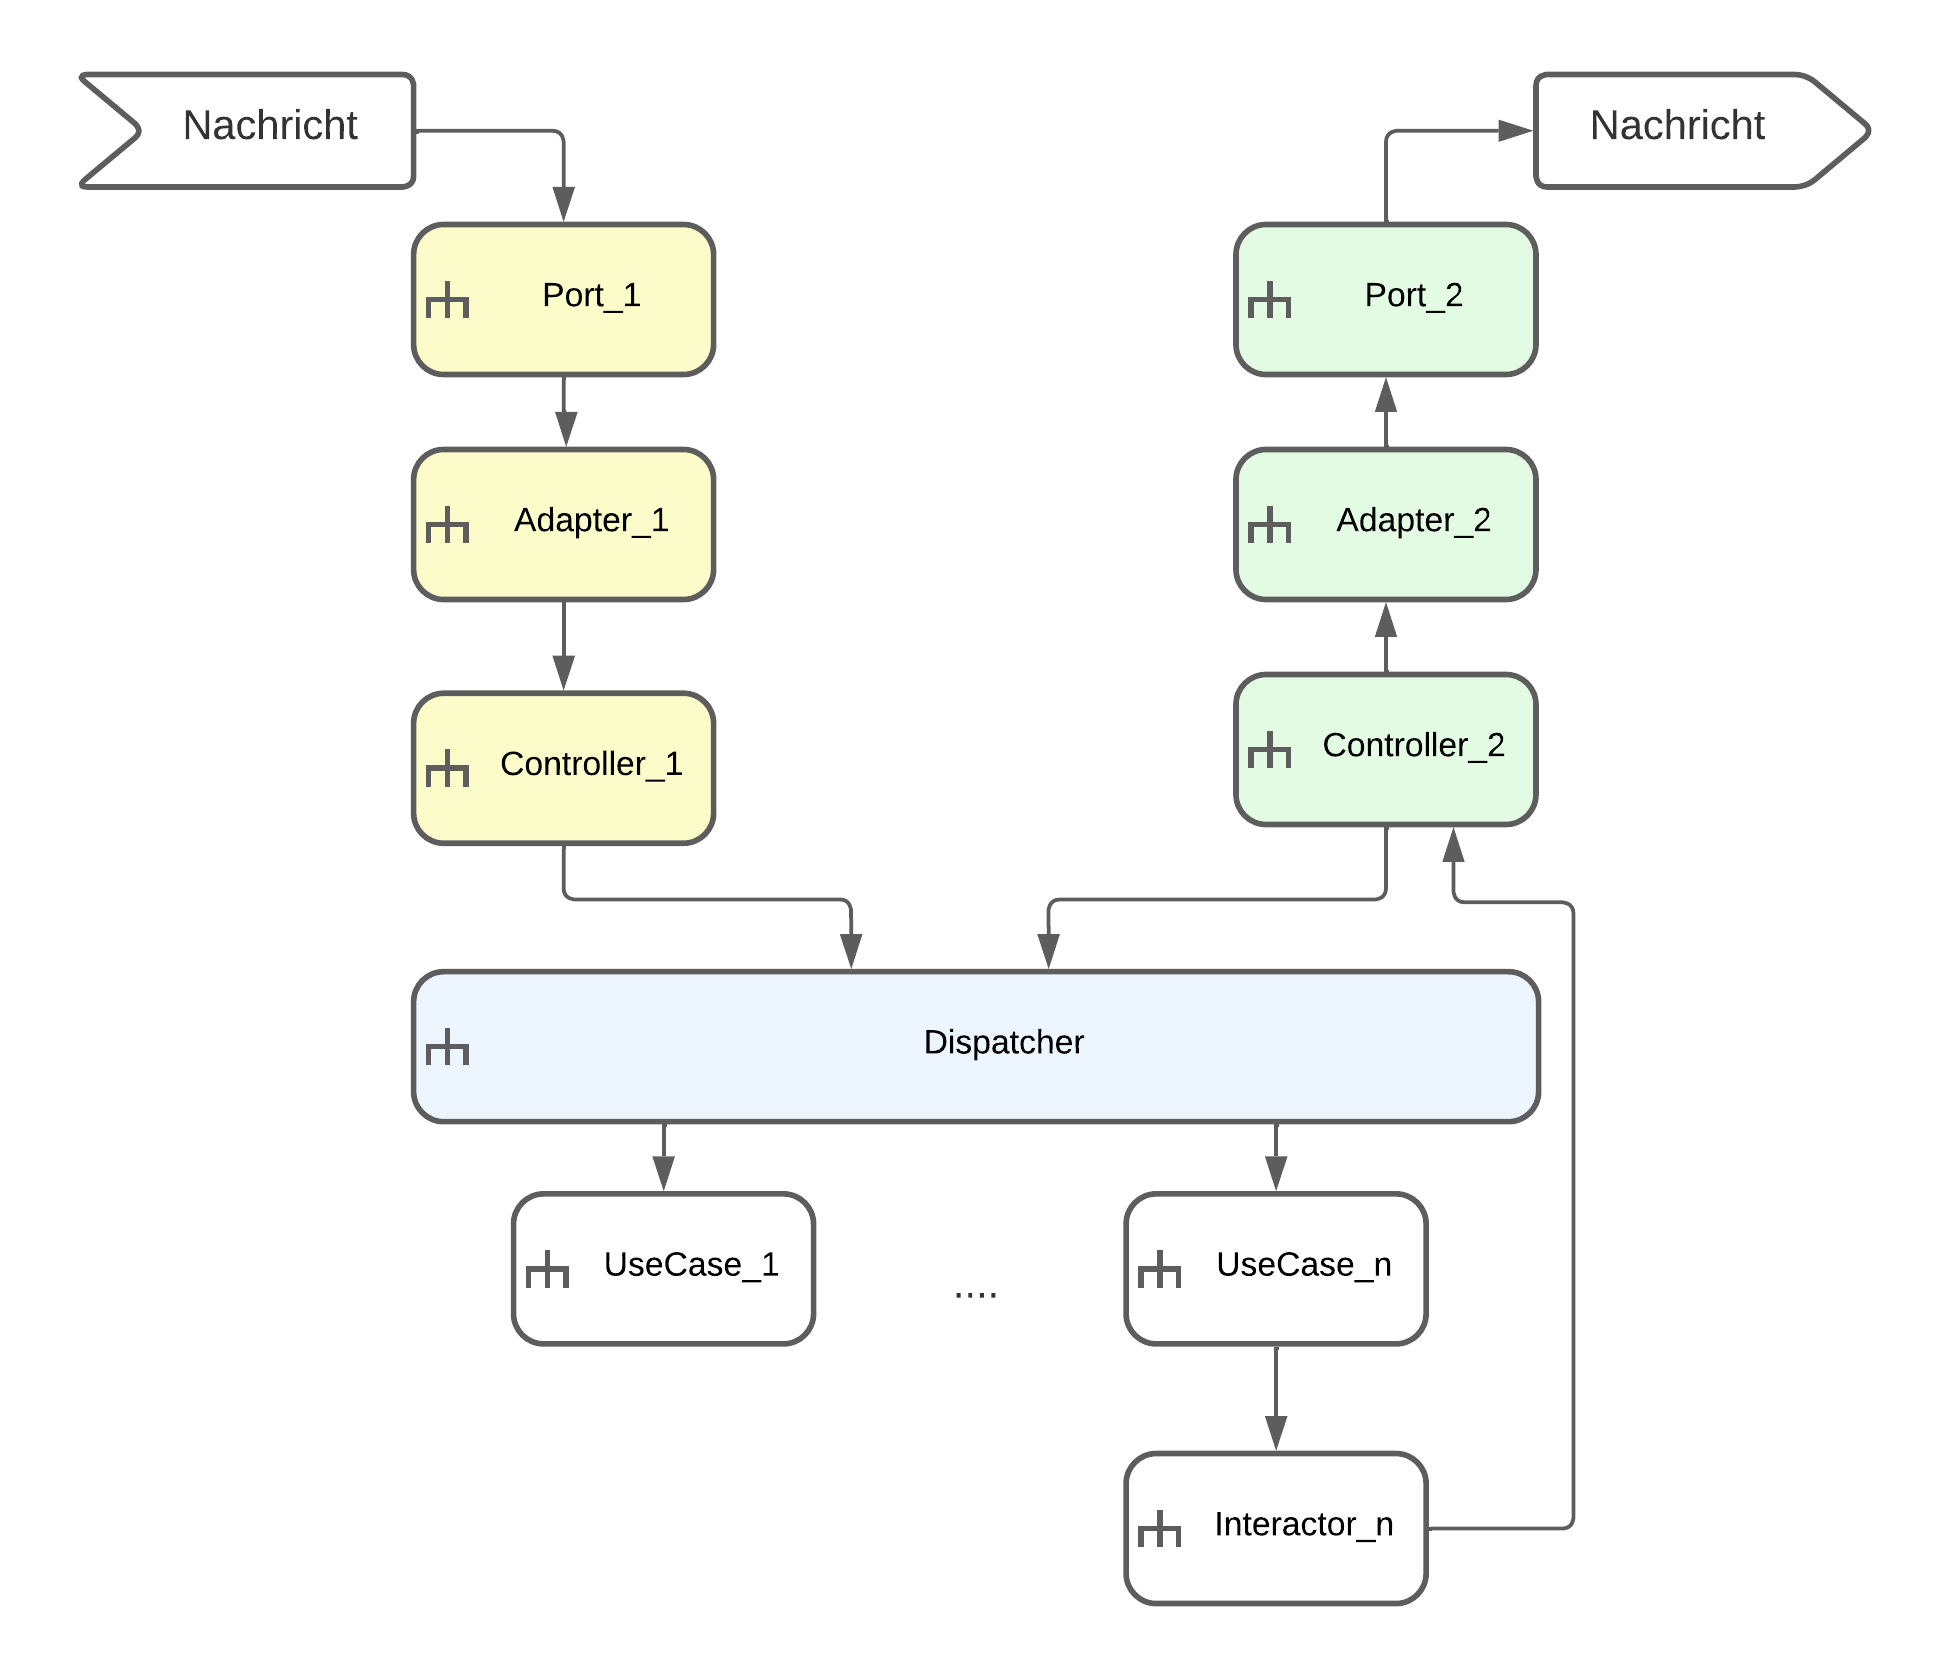
\includegraphics[width=12cm]{./images/FullDataFlow.png}
         \caption[Kompletter Datenfluss]{Kompletter Datenfluss \footnotemark}
         \label{fig:FullDataFlow}
    \end{figure}
    \footnotetext{Eigene Quelle}

    \newpage
    \subsubsection{Parallelismus}
    evtl. auf Funktionales Programmieren hinweisen.
    In der beschriebenen Struktur lassen sich folgende Prozesse parallel ausführen:
    \begin{itemize}
        \item Jede Controller-Adapter-Port Komponente
        \item Dispatcher
        \item Jedes aktives UseCase
    \end{itemize}

    \subsubsection{Auswahl der Datenbank}
    \subsubsection{Dependency Rule}
    \subsubsection{Unterschied zu Layered Architektur}
    \subsubsection{Implementierung der Testbarkeit}
    - Humble Objects
    \subsubsection{Dependency Injection}
    \label{DependencyInjection}
    In der Abbildung \ref{fig:dateflowVScodedep} sieht man ein Beispiel von einer Anwendung, die die von der Konsole ankommenden Zahlen quadriert und das Ergebnis zurückgibt.
    
    \begin{figure}[H]
        \centering
        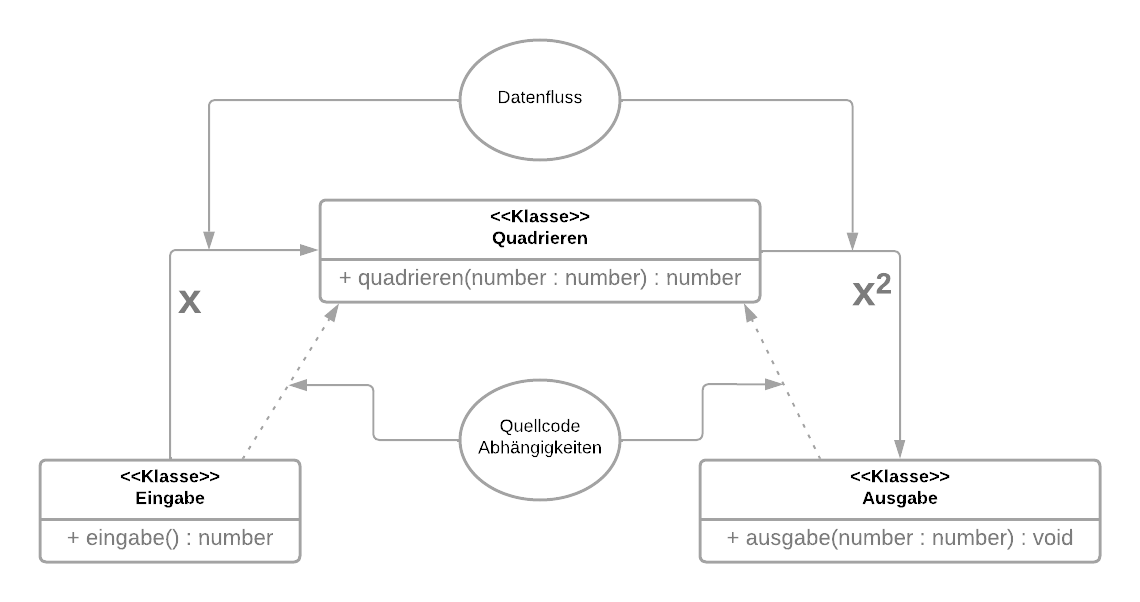
\includegraphics[width=1\textwidth]{./images/DepInj_1.png}
        \caption{Datenfluss und Quellcode Abhängigkeiten}
        \label{fig:dateflowVScodedep}
        \source{Eigene Quelle}
    \end{figure}

    Die Funktion \textbf{Quadrieren} ist in dem Fall befindet sich auf einem höheren Niveau als Eingabe und Ausgabe, 
    da das Quadrieren einer Zahl soll unabhängig von der Eingabe und Ausgabe sein.

    Würde man aber bei der Ausgabe die Eingabeparameter von \textbf{number} auf \textbf{string} ändern, 
    so müsste man auch die Ausgabe von Quadrieren von \textbf{number} auf \textbf{string} ändern.
    Dies könnte auch eine weitere Kette an Anderungen im Programm auslösen. 
    Zum Beispiel müssen auch die Unittests von \textbf{Quadrieren} geändert werden.
    Somit ist \textbf{Quadrieren} abhängig von der \textbf{Ausgabe}

    Das Problem lässt sich mittels Dependency Injection lösen.
    In OOP Sprachen kann man dafür ``Interface'' benutzen.

    Die Lösung wurde dann so aussehen. 
    \begin{figure}[H]
        \centering
        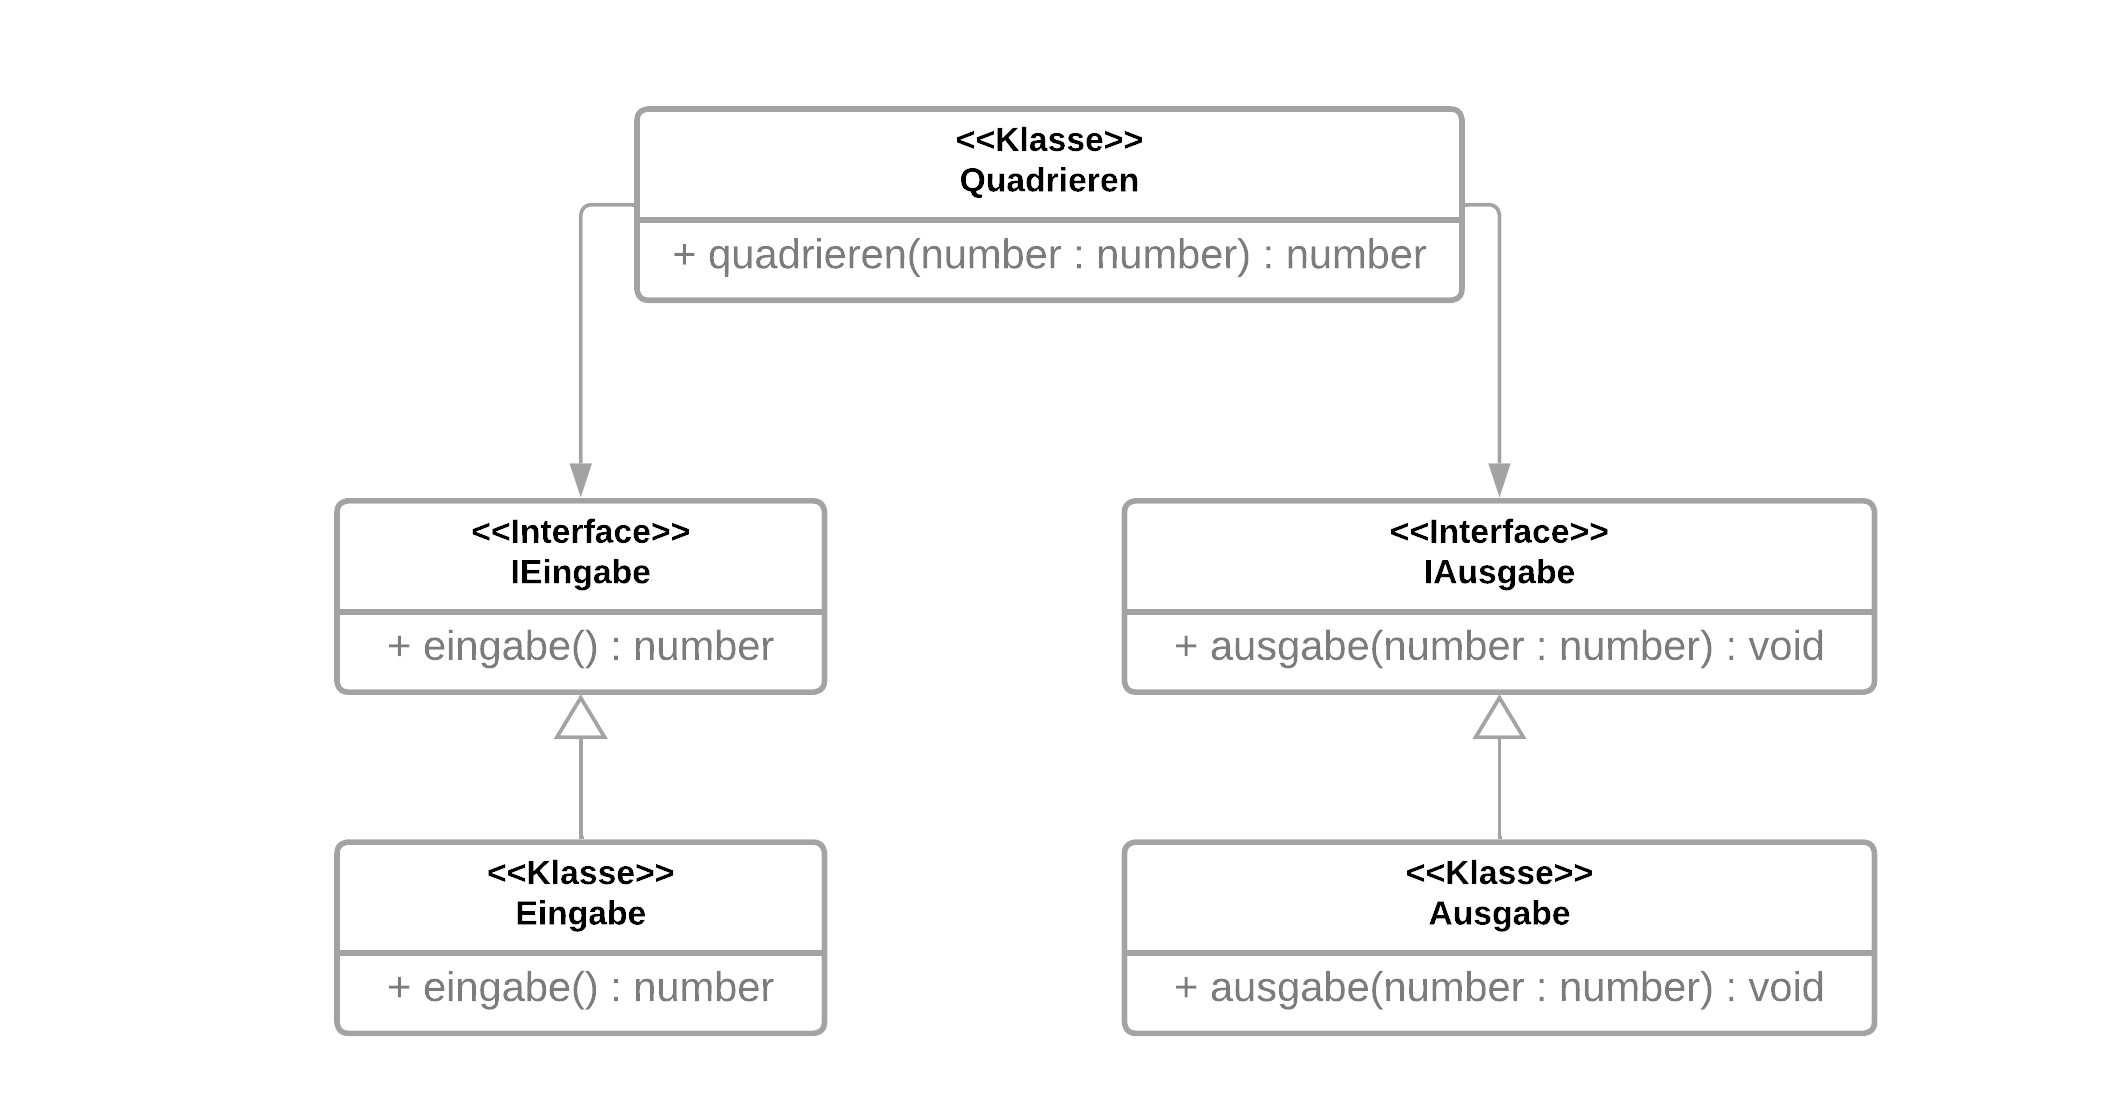
\includegraphics[width=1\textwidth]{./images/DepInj_2.png}
        \caption{Entkopplung der Abhängigkeiten}
        \label{fig:flow around cylinder}
        \source{Eigene Quelle}
    \end{figure}

    Dies lässt sich mit \textbf{Interface} (für OOP Sprachen) umsetzen, 
    in dem es frühestens bei der Initialisiereung der \textbf{Quadrieren} 
    Klasse das jeweilige Eingabe und Ausgabe Objekt übergeben wird.

    Somit lässt sich die Funktion \textbf{Quadrieren} mit gefälschten Eingabe- und Ausgabeklasse mit Unit tests getestet werden.

    Wenn man alle Klassen über Interface miteinander verbindet, 
    ist es möglich, dass die Umgebung von jeder einzelnen Klasse bei den Unittests gefälscht
    wird und somit das Schreiben von Unittests sehr einfach wird. 

    Interfaces können sich natürlich auch ändern und dann muss man auch alle davon betroffenen Objekte entsprechend ändern, 
    jedoch das passiert deutlich seltener als Änderung einer Klasse.

    Auch mit Dependency Injection lassen sich externe Schnittstellen wie Datenbank oder Netzwerkschnittstellen schnell austauschen, 
    denn man muss nur eine Klasse schreiben, die das Interface implementiert.

    \newpage
    \subsection{Erweiterung der Funktionalitäten}
    Wie am Anfang angedeutet wurde, ein wichtiges Ziel der Architectur ist die leichte Erweiterung der jeglichen Funktionalitäten der 
    Anwendung. In dem Kapitel werden mehrere Szenarien betrachtet und entsprechend beschrieben, an welchen Stellen was geändert bzw.
    hinzugefügt werden soll. Bei allen Änderungen darf man nicht vergessen, dass sie entsprechend im Programm initalisiert werden.
    (z.B. eine entsprechende Instanz gestartet wird usw.)
    
    \subsubsection{Verhalten für ein Ereignis erweitern}
    \label{Verhalten für ein Ereignis erweitern}
    Bei diesem Szenario, geht man davon aus das ein Ereignis an Dispatcher ankommt und entspechend an alle dafür 
    verantwortlichen UseCases weiterleitet. 
    Es gibt hier zwei Möglichkeiten:
    \begin{enumerate}
        \item bestehendes UseCase um die neue Funktionalität erweitern.
        \item neues UseCase erstellen, das das gleiche Ereignis handelt.
    \end{enumerate}

    Mit der ersten Möglichkeit hat man das komplete Verhalten für ein Ereignis an einem Ort und mit Unittests abdecken.

    Die zweite Möglichkeit streut das Verhalten für ein Ereignis im Projekt, was eine besere Lesbarkeit des jeweiligen Teils erhöht,
    jedoch die Schwierigkeit bringt alle solche Teile im Projekt zu finden. Das Gesamtverhalten lässt sich erst mittels
    einem Integrationtest abdecken, was eine mögliche Fehlersuche erschweren kann. 
    Für den Fall, dass das neue Verhalten unabhängig von dem bestehenden Verhalten ablaufen soll ist es eine gute Möglichkeit.
    
    \subsubsection{Eine bestehende Schnittstelle um 1 Ereignis erweitern}
    In dem Fall wird nur der Datenweg vom \textbf{Port}-\textbf{Adapter}-\textbf{Controller} betrachtet und welche Änderungen,
    da entsprechend gemacht werden müssen.

    Der Weg vom \textbf{Port} zum \textbf{Controller}

    \begin{itemize}
        \item \textbf{Port} in dem Teil sollen keine Änderungen gemacht werden.
        \item \textbf{Adapter} in dem Teil soll das Validieren des ankommenden Ereignisses hinzugefügt werden. Normalerweise würde 
        das Ereignis als ein unbekanntes Ereignis markiert und dann weitergeleitet.
        \item \textbf{Controller} in dem Teil sollen keine Änderungen gemacht werden.
    \end{itemize}

    Der Weg vom \textbf{Controller} zum \textbf{Port}
    \begin{itemize}
        \item \textbf{Controller} das Absenden soll ermöglicht werden, evtl. auch ein \textbf{Interactor} hinzufügen
        \item \textbf{Adapter} um das Umwandeln des Ereignisses soll erweitert werden.
        \item \textbf{Port} in dem Teil sollen keine Änderungen gemacht werden.
    \end{itemize}

    \newpage
    \subsubsection{Neue Schnittstelle hinzufügen}
    Wenn man eine neue Schnittstelle hinzufügen möchte, muss man 3 neue Teile erstellen.
    \begin{itemize}
        \item \textbf{Port}
        \item \textbf{Adapter}
        \item \textbf{Controller} evtl. auch \textbf{Interactoren} hinzufügen
    \end{itemize}

    \subsubsection{Das Verhalten für ein neues Ereignis hinzufügen}
    Der Ablauf in dem Fall ist gleich dem Ablauf der zweiten Möglichkeit in dem Teil \ref{Verhalten für ein Ereignis erweitern}.
    Man hat dabei keine beschriebenen Nachteile, die in dem Kapitel beschrieben sind.
    
    \newpage
    \subsection{Anbindung in eine andere Anwendung als eine Komponente}
    Nicht jede Software wird als Standalone Anwendung ausgeführt, es kann auch passieren, dass man 
    erst ein Kern umsetzt, die dann in jeweiligen Anwendungen entsprechend angepasst werden 
    oder es handelt sich nur um eine Komponente für die andere Anwednung.
    Eine Analogie aus OOP wäre eine Abstrakte Klasse.

    Grundsätzlich kann man die Abbildung \ref{fig:sp2d} folgendeweise vereinfachen:
    \begin{figure}[H]
        \centering
        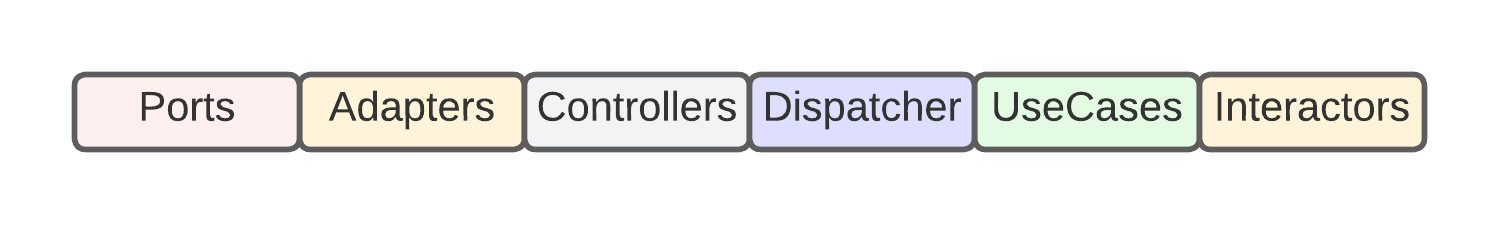
\includegraphics[width=1\textwidth]{./images/SimpliedArchitecture.png}
        \caption{Vereinfachte Darstellung}
        \label{fig:SimpliedArchitecture}
        \source{Eigene Quelle}
    \end{figure}

    Und bei einer Standalone Anwendung gibt es eine Main-Methode, die diese Struktrur erstellt.
    \begin{figure}[H]
        \centering
        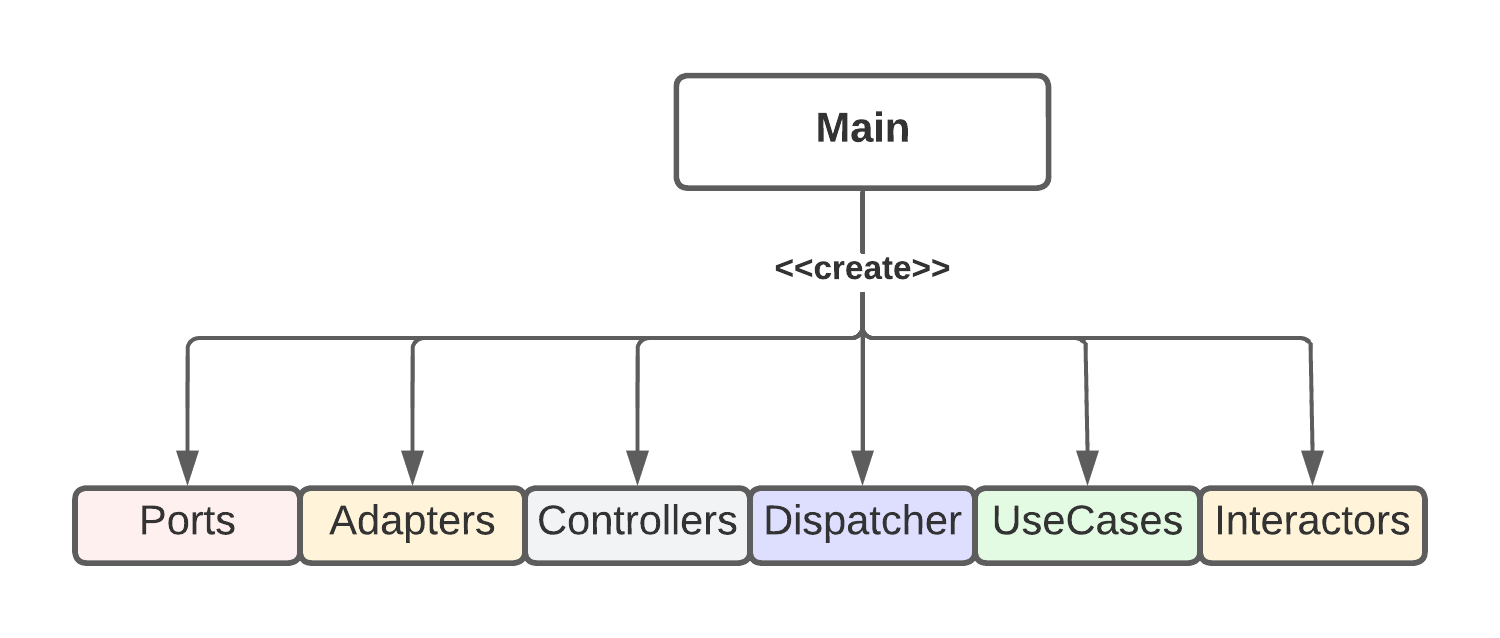
\includegraphics[width=1\textwidth]{./images/Architecture as Standalone.png}
        \caption{Vereinfachte Darstellung einer Standalone Anwendung}
        \label{fig:SimpliedArchitectureAsStandalone}
        \source{Eigene Quelle}
    \end{figure}
    
    Der Datenfluss lässt sich so darstellen:
    \begin{figure}[H]
        \centering
        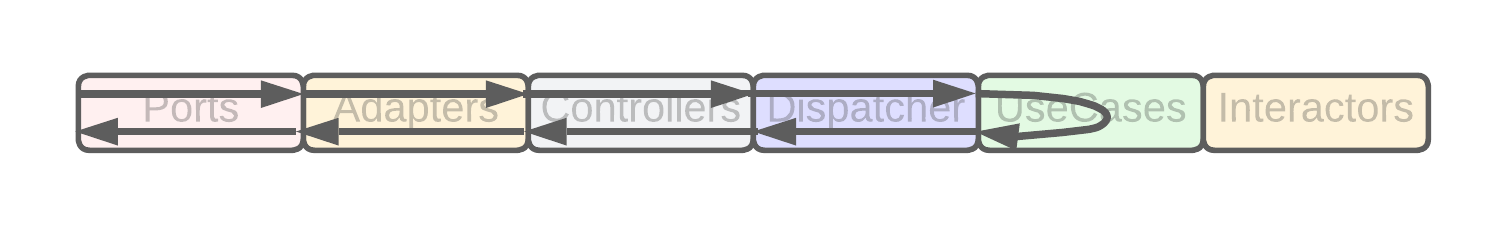
\includegraphics[width=1\textwidth]{./images/Dataflow.png}
        \caption{Vereinfachte Darstellung einer Standalone Anwendung}
        \label{fig:SimpliedArchitectureDataflow}
        \source{Eigene Quelle}
    \end{figure}

    \newpage
    Wenn man es als Komponente in einer anderen Anwendung benutzen möchte, braucht die Struktur eine Facade, damit man 
    auf "wichtige Teile" der Komponente zugreifen kann und der Rest verborgen bleibt. 
    Die Facade baut die gesamte Struktur der Komponente auf.

    So sieht eine fertige Komponente aus, die man in die anderen Anwendungen integrieren kann:
    \begin{figure}[H]
        \centering
        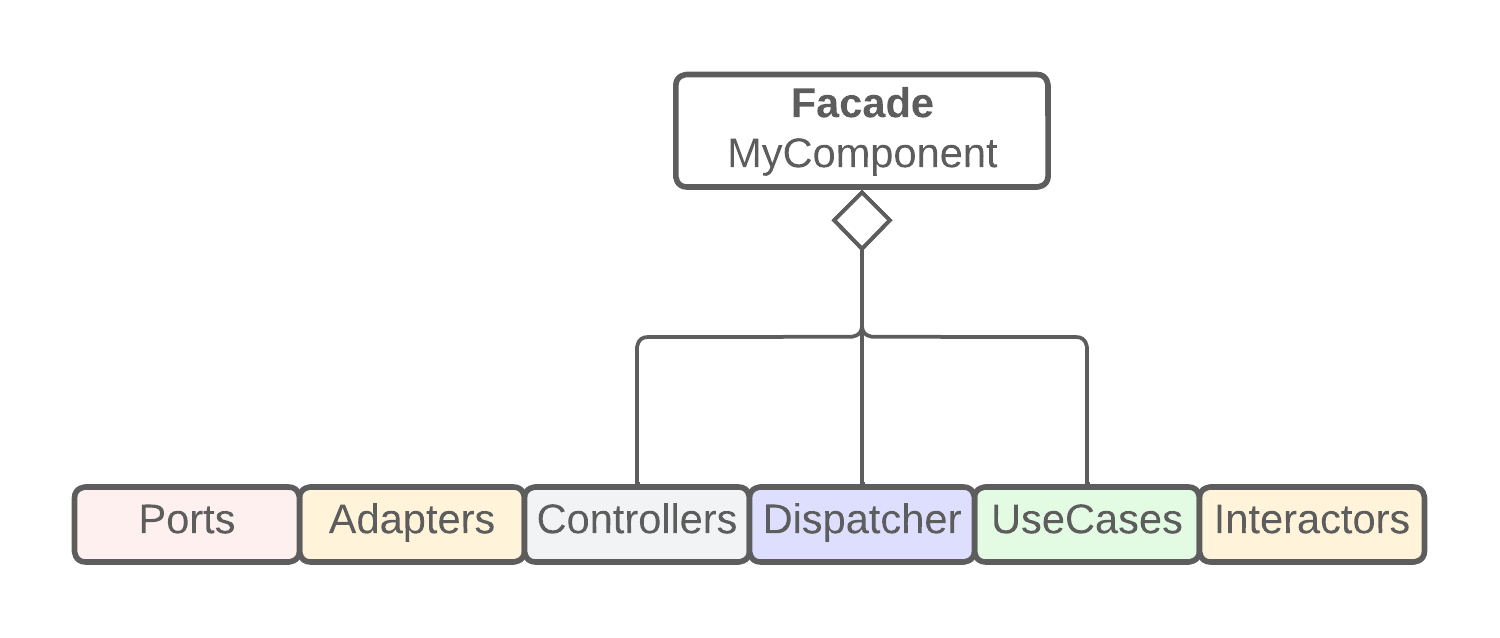
\includegraphics[width=1\textwidth]{./images/Architecture as Facade.png}
        \caption{Vereinfacte Darstellung der Architektur als Komponente}
        \label{fig:SimpliedArchitectureAsKomponent}
        \source{Eigene Quelle}
    \end{figure}

    Auf der Darstellung \ref{fig:SimpliedArchitectureAsKomponent} sieht man, dass die Anwendung nur den Zugriff auf drei Teile der Komponente hat.
    Das sind:
    \begin{itemize}
        \item \textbf{Controllers} - um die Zustände des jeweiligen Controllers abfragen und ändern.
        \item \textbf{Dispatcher} - um alle Ereignise in der Komponente abzufangen.
        \item \textbf{UseCases} - um das Verhalten auf gewisse Ereignise ändern zu können.
    \end{itemize}

    Die Komponente kann bestimmte Ereignise selber abarbeiten und die Anwendung davon gar nicht informieren oder
    das Ereignis weiterleiten, dass es von der Anwednung selbst abarbeitet wird.
    Die Komponente wird von der eigentlichen Anwendung unabhängig entwickelt, somit wird es passieren, dass
    der Datentyp des Ereignisses von der Komponente nicht mit dem Datentyp der Anwendung übereinstimmt und deswegen muss noch durch den entsprechenden Adapter angepasst werden.
    Das bedeutet, dass die Komponente wird nur von dem \textbf{Port} der jeweiligen Anwendung benutzt wird.

    \newpage
    Die Vereinfacte Darstellung der Anwendung mit der Komponente:
    \begin{figure}[H]
        \centering
        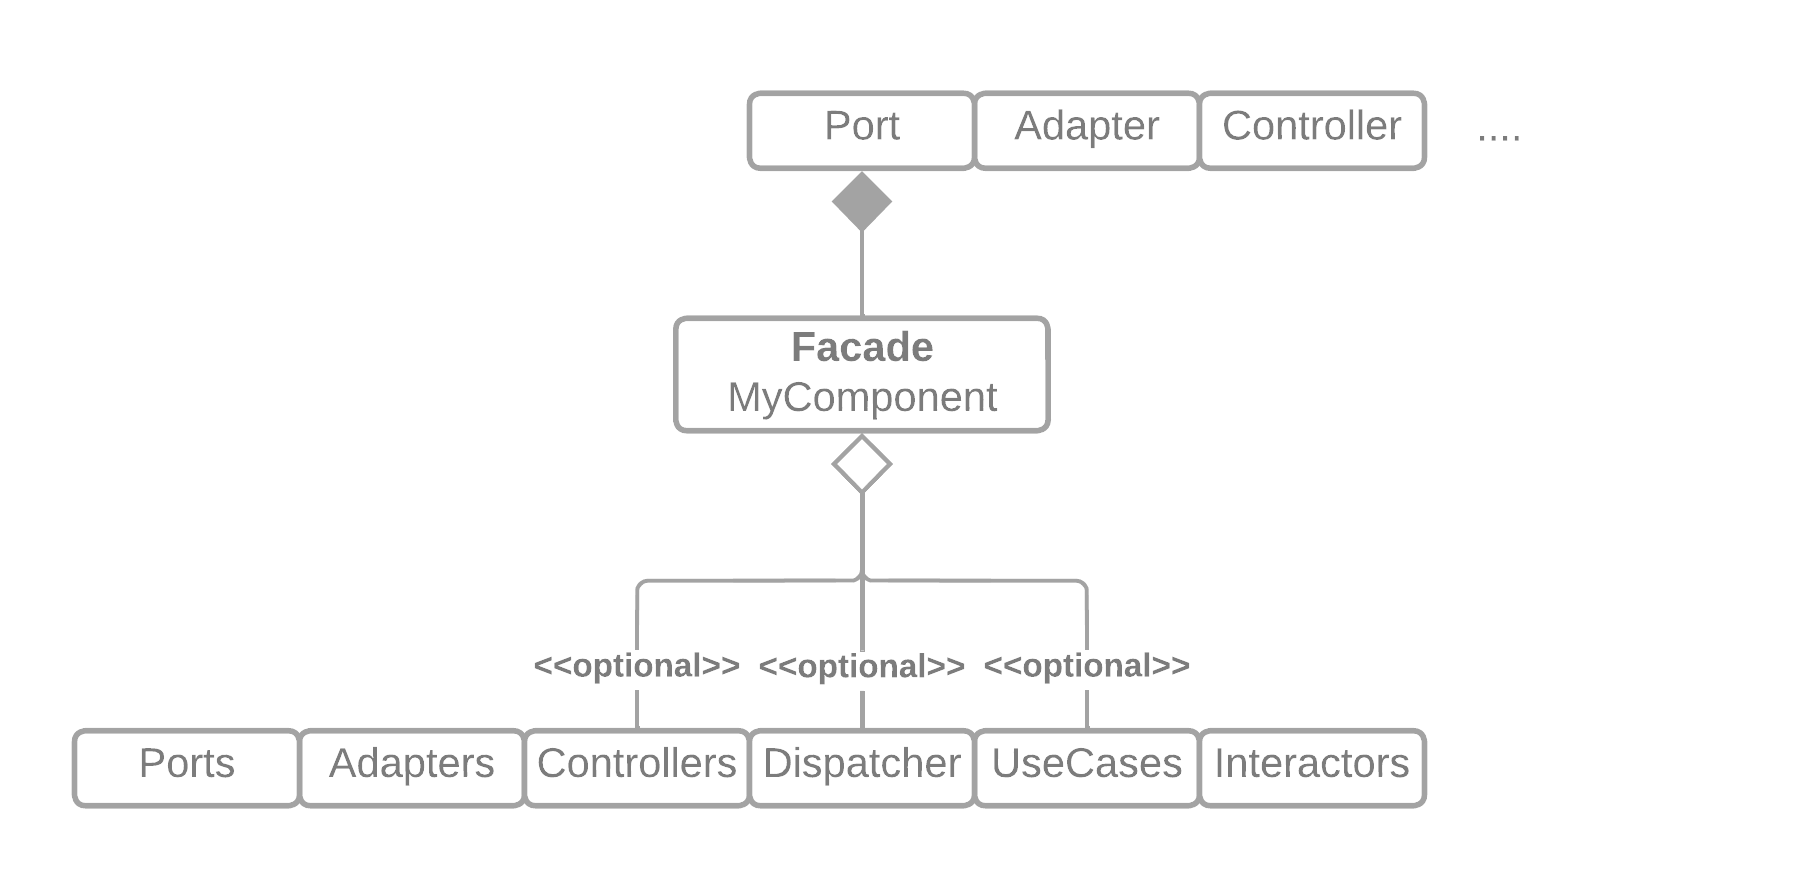
\includegraphics[width=1\textwidth]{./images/Architecture as Component.png}
        \caption{Vereinfacte Darstellung einer Standalone Anwendung mit der Komponente}
        \label{fig:SimpliedArchitectureAsStandaloneWithComponent}
        \source{Eigene Quelle}
    \end{figure}

    Der Datenfluss in der Anwendung würde wie folgt aussehen:
    \begin{figure}[H]
        \centering
        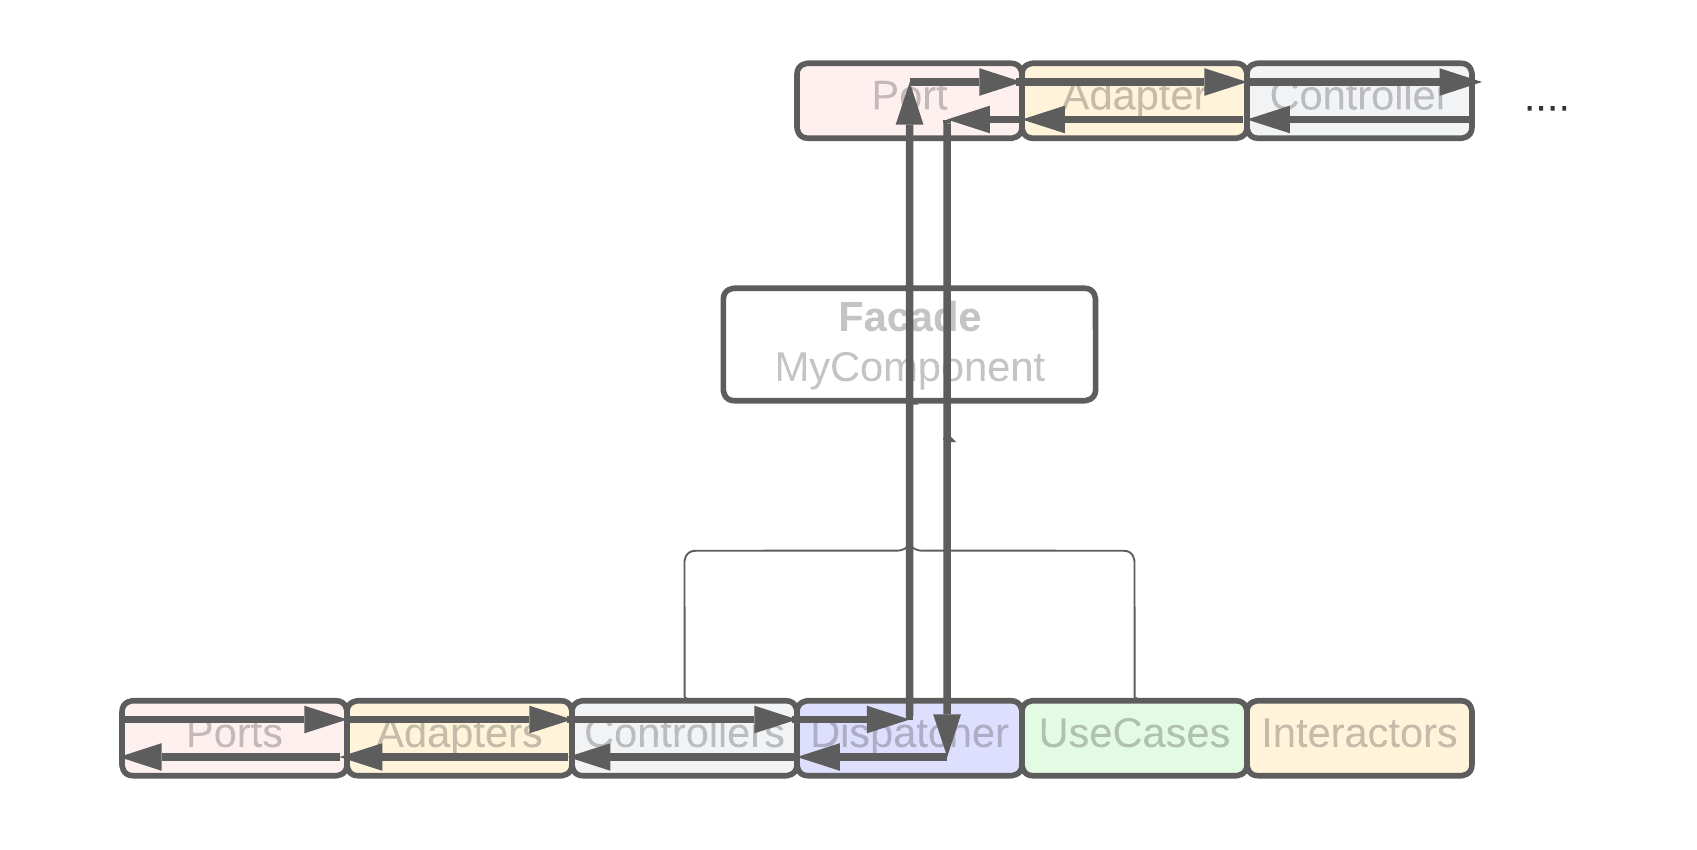
\includegraphics[width=1\textwidth]{./images/Dataflow as Component with inform.png}
        \caption{Vereinfacte Darstellung des Datenflusses in einer Anwendung mit Komponente}
        \label{fig:SimpliedDataflowWithComponent}
        \source{Eigene Quelle}
    \end{figure}

\newpage



% Example section added from an external tex-file, here located in ./Sections/
\import{./Sections/}{Aufgabestellung}

\import{./Sections/}{Loesung}


% Beschreibung der gewünschten Implementierung
\newpage
\import{./Sections/}{Bestinterface}

% Beschreibung der Implementierung der Software
\newpage
\import{./Sections/}{Implementierung}

\section{Übersichtsdiagramm}

% Example section added directly into the main-file
\section{Conclusion}
\textit{But the fact that some geniuses were laughed at does not imply that all who are laughed at are geniuses. They laughed at Columbus, they laughed at Fulton, they laughed at the Wright Brothers. But they also laughed at Bozo the Clown} -  \textcite{sagan_1993}.

% Printing bibliography
\newpage
\printbibliography[heading = bibintoc, title = Bibliography]    % 'bibintoc' inserts our bibliography into the table of contents

% Inserting appendix with separate settings
\addappendix
\import{./Appendices/}{example_appendix}

% End of document
\end{document}
